\documentclass[10pt, oneside]{article} 
\usepackage{amsmath, amsthm, amssymb, calrsfs, wasysym, verbatim, bbm, color, graphics, geometry, esint, float}


\geometry{tmargin=.75in, bmargin=.75in, lmargin=.75in, rmargin = .75in}  

\newcommand{\bbR}{\mathbb{R}}
\newcommand{\bbC}{\mathbb{C}}
\newcommand{\bbZ}{\mathbb{Z}}
\newcommand{\bbN}{\mathbb{N}}
\newcommand{\bbQ}{\mathbb{Q}}
\newcommand{\Cdot}{\boldsymbol{\cdot}}
\newcommand{\scA}{\mathscr{A}}
\newcommand{\curl}{\text{curl}}

\theoremstyle{definition}
\newtheorem{exmp}{Example}[section]
\newtheorem{thm}{Theorem}
\newtheorem{defn}{Definition}
\newtheorem{prop}{Proposition}
\newtheorem{conv}{Convention}
\newtheorem{rem}{Remark}
\newtheorem{lem}{Lemma}
\newtheorem{cor}{Corollary}
% Copyright 2021 Paolo Adajar (padajar.com, paoloadajar@mit.edu)
% 
% Permission is hereby granted, free of charge, to any person obtaining a copy of this software and associated documentation files (the "Software"), to deal in the Software without restriction, including without limitation the rights to use, copy, modify, merge, publish, distribute, sublicense, and/or sell copies of the Software, and to permit persons to whom the Software is furnished to do so, subject to the following conditions:
%
% The above copyright notice and this permission notice shall be included in all copies or substantial portions of the Software.
% 
% THE SOFTWARE IS PROVIDED "AS IS", WITHOUT WARRANTY OF ANY KIND, EXPRESS OR IMPLIED, INCLUDING BUT NOT LIMITED TO THE WARRANTIES OF MERCHANTABILITY, FITNESS FOR A PARTICULAR PURPOSE AND NONINFRINGEMENT. IN NO EVENT SHALL THE AUTHORS OR COPYRIGHT HOLDERS BE LIABLE FOR ANY CLAIM, DAMAGES OR OTHER LIABILITY, WHETHER IN AN ACTION OF CONTRACT, TORT OR OTHERWISE, ARISING FROM, OUT OF OR IN CONNECTION WITH THE SOFTWARE OR THE USE OR OTHER DEALINGS IN THE SOFTWARE.

\usepackage{fullpage}
\usepackage{enumitem}
\usepackage{amsfonts, amssymb, amsmath,amsthm}
\usepackage{mathtools}
\usepackage[pdftex, pdfauthor={\name}, pdftitle={\classnum~\assignment}]{hyperref}
\usepackage[dvipsnames]{xcolor}
\usepackage{bbm}
\usepackage{graphicx}
\usepackage{mathrsfs}
\usepackage{pdfpages}
\usepackage{tabularx}
\usepackage{pdflscape}
\usepackage{makecell}
\usepackage{booktabs}
\usepackage{natbib}
\usepackage{caption}
\usepackage{subcaption}
\usepackage{physics}
\usepackage[many]{tcolorbox}
\usepackage{version}
\usepackage{ifthen}
\usepackage{cancel}
\usepackage{listings}
\usepackage{courier}

\usepackage{tikz}
\usepackage{istgame}

\hypersetup{
	colorlinks=true,
	linkcolor=blue,
	filecolor=magenta,
	urlcolor=blue,
}

\setlength{\parindent}{0mm}
\setlength{\parskip}{2mm}

\setlist[enumerate]{label=({\alph*})}
\setlist[enumerate, 2]{label=({\roman*})}

\allowdisplaybreaks[1]

\newcommand{\psetheader}{
	\ifthenelse{\isundefined{\collaborators}}{
		\begin{center}
			{\setlength{\parindent}{0cm} \setlength{\parskip}{0mm}
				
				{\textbf{\classnum~\semester:~\assignment} \hfill \name}
				
				\subject \hfill \href{mailto:\email}{\tt \email}
				
				Instructor(s):~\instructors \hfill Due Date:~\duedate	
				
				\hrulefill}
		\end{center}
	}{
		\begin{center}
			{\setlength{\parindent}{0cm} \setlength{\parskip}{0mm}
				
				{\textbf{\classnum~\semester:~\assignment} \hfill \name\footnote{Collaborator(s): \collaborators}}
				
				\subject \hfill \href{mailto:\email}{\tt \email}
				
				Instructor(s):~\instructors \hfill Due Date:~\duedate	
				
				\hrulefill}
		\end{center}
	}
}

\renewcommand{\thepage}{\classnum~\assignment \hfill \arabic{page}}

\makeatletter
\def\points{\@ifnextchar[{\@with}{\@without}}
\def\@with[#1]#2{{\ifthenelse{\equal{#2}{1}}{{[1 point, #1]}}{{[#2 points, #1]}}}}
\def\@without#1{\ifthenelse{\equal{#1}{1}}{{[1 point]}}{{[#1 points]}}}
\makeatother

\newtheoremstyle{theorem-custom}%
{}{}%
{}{}%
{\itshape}{.}%
{ }%
{\thmname{#1}\thmnumber{ #2}\thmnote{ (#3)}}

\theoremstyle{theorem-custom}

\newtheorem{theorem}{Theorem}
\newtheorem{lemma}[theorem]{Lemma}
\newtheorem{example}[theorem]{Example}

\newenvironment{problem}[1]{\color{black} #1}{}

\newenvironment{solution}{%
	\leavevmode\begin{tcolorbox}[breakable, colback=green!5!white,colframe=green!75!black, enhanced jigsaw] \proof[\scshape Solution:] \setlength{\parskip}{2mm}%
	}{\renewcommand{\qedsymbol}{$\blacksquare$} \endproof \end{tcolorbox}}

\newenvironment{reflection}{\begin{tcolorbox}[breakable, colback=black!8!white,colframe=black!60!white, enhanced jigsaw, parbox = false]\textsc{Reflections:}}{\end{tcolorbox}}

\newcommand{\qedh}{\renewcommand{\qedsymbol}{$\blacksquare$}\qedhere}

\definecolor{mygreen}{rgb}{0,0.6,0}
\definecolor{mygray}{rgb}{0.5,0.5,0.5}
\definecolor{mymauve}{rgb}{0.58,0,0.82}

% from https://github.com/satejsoman/stata-lstlisting
% language definition
\lstdefinelanguage{Stata}{
	% System commands
	morekeywords=[1]{regress, reg, summarize, sum, display, di, generate, gen, bysort, use, import, delimited, predict, quietly, probit, margins, test},
	% Reserved words
	morekeywords=[2]{aggregate, array, boolean, break, byte, case, catch, class, colvector, complex, const, continue, default, delegate, delete, do, double, else, eltypedef, end, enum, explicit, export, external, float, for, friend, function, global, goto, if, inline, int, local, long, mata, matrix, namespace, new, numeric, NULL, operator, orgtypedef, pointer, polymorphic, pragma, private, protected, public, quad, real, return, rowvector, scalar, short, signed, static, strL, string, struct, super, switch, template, this, throw, transmorphic, try, typedef, typename, union, unsigned, using, vector, version, virtual, void, volatile, while,},
	% Keywords
	morekeywords=[3]{forvalues, foreach, set},
	% Date and time functions
	morekeywords=[4]{bofd, Cdhms, Chms, Clock, clock, Cmdyhms, Cofc, cofC, Cofd, cofd, daily, date, day, dhms, dofb, dofC, dofc, dofh, dofm, dofq, dofw, dofy, dow, doy, halfyear, halfyearly, hh, hhC, hms, hofd, hours, mdy, mdyhms, minutes, mm, mmC, mofd, month, monthly, msofhours, msofminutes, msofseconds, qofd, quarter, quarterly, seconds, ss, ssC, tC, tc, td, th, tm, tq, tw, week, weekly, wofd, year, yearly, yh, ym, yofd, yq, yw,},
	% Mathematical functions
	morekeywords=[5]{abs, ceil, cloglog, comb, digamma, exp, expm1, floor, int, invcloglog, invlogit, ln, ln1m, ln, ln1p, ln, lnfactorial, lngamma, log, log10, log1m, log1p, logit, max, min, mod, reldif, round, sign, sqrt, sum, trigamma, trunc,},
	% Matrix functions
	morekeywords=[6]{cholesky, coleqnumb, colnfreeparms, colnumb, colsof, corr, det, diag, diag0cnt, el, get, hadamard, I, inv, invsym, issymmetric, J, matmissing, matuniform, mreldif, nullmat, roweqnumb, rownfreeparms, rownumb, rowsof, sweep, trace, vec, vecdiag, },
	% Programming functions
	morekeywords=[7]{autocode, byteorder, c, _caller, chop, abs, clip, cond, e, fileexists, fileread, filereaderror, filewrite, float, fmtwidth, has_eprop, inlist, inrange, irecode, matrix, maxbyte, maxdouble, maxfloat, maxint, maxlong, mi, minbyte, mindouble, minfloat, minint, minlong, missing, r, recode, replay, return, s, scalar, smallestdouble,},
	% Random-number functions
	morekeywords=[8]{rbeta, rbinomial, rcauchy, rchi2, rexponential, rgamma, rhypergeometric, rigaussian, rlaplace, rlogistic, rnbinomial, rnormal, rpoisson, rt, runiform, runiformint, rweibull, rweibullph,},
	% Selecting time-span functions
	morekeywords=[9]{tin, twithin,},
	% Statistical functions
	morekeywords=[10]{betaden, binomial, binomialp, binomialtail, binormal, cauchy, cauchyden, cauchytail, chi2, chi2den, chi2tail, dgammapda, dgammapdada, dgammapdadx, dgammapdx, dgammapdxdx, dunnettprob, exponential, exponentialden, exponentialtail, F, Fden, Ftail, gammaden, gammap, gammaptail, hypergeometric, hypergeometricp, ibeta, ibetatail, igaussian, igaussianden, igaussiantail, invbinomial, invbinomialtail, invcauchy, invcauchytail, invchi2, invchi2tail, invdunnettprob, invexponential, invexponentialtail, invF, invFtail, invgammap, invgammaptail, invibeta, invibetatail, invigaussian, invigaussiantail, invlaplace, invlaplacetail, invlogistic, invlogistictail, invnbinomial, invnbinomialtail, invnchi2, invnF, invnFtail, invnibeta, invnormal, invnt, invnttail, invpoisson, invpoissontail, invt, invttail, invtukeyprob, invweibull, invweibullph, invweibullphtail, invweibulltail, laplace, laplaceden, laplacetail, lncauchyden, lnigammaden, lnigaussianden, lniwishartden, lnlaplaceden, lnmvnormalden, lnnormal, lnnormalden, lnwishartden, logistic, logisticden, logistictail, nbetaden, nbinomial, nbinomialp, nbinomialtail, nchi2, nchi2den, nchi2tail, nF, nFden, nFtail, nibeta, normal, normalden, npnchi2, npnF, npnt, nt, ntden, nttail, poisson, poissonp, poissontail, t, tden, ttail, tukeyprob, weibull, weibullden, weibullph, weibullphden, weibullphtail, weibulltail,},
	% String functions 
	morekeywords=[11]{abbrev, char, collatorlocale, collatorversion, indexnot, plural, plural, real, regexm, regexr, regexs, soundex, soundex_nara, strcat, strdup, string, strofreal, string, strofreal, stritrim, strlen, strlower, strltrim, strmatch, strofreal, strofreal, strpos, strproper, strreverse, strrpos, strrtrim, strtoname, strtrim, strupper, subinstr, subinword, substr, tobytes, uchar, udstrlen, udsubstr, uisdigit, uisletter, ustrcompare, ustrcompareex, ustrfix, ustrfrom, ustrinvalidcnt, ustrleft, ustrlen, ustrlower, ustrltrim, ustrnormalize, ustrpos, ustrregexm, ustrregexra, ustrregexrf, ustrregexs, ustrreverse, ustrright, ustrrpos, ustrrtrim, ustrsortkey, ustrsortkeyex, ustrtitle, ustrto, ustrtohex, ustrtoname, ustrtrim, ustrunescape, ustrupper, ustrword, ustrwordcount, usubinstr, usubstr, word, wordbreaklocale, worcount,},
	% Trig functions
	morekeywords=[12]{acos, acosh, asin, asinh, atan, atanh, cos, cosh, sin, sinh, tan, tanh,},
	morecomment=[l]{//},
	% morecomment=[l]{*},  // `*` maybe used as multiply operator. So use `//` as line comment.
	morecomment=[s]{/*}{*/},
	% The following is used by macros, like `lags'.
	morestring=[b]{`}{'},
	% morestring=[d]{'},
	morestring=[b]",
	morestring=[d]",
	% morestring=[d]{\\`},
	% morestring=[b]{'},
	sensitive=true,
}

\lstset{ 
	backgroundcolor=\color{white},   % choose the background color; you must add \usepackage{color} or \usepackage{xcolor}; should come as last argument
	basicstyle=\footnotesize\ttfamily,        % the size of the fonts that are used for the code
	breakatwhitespace=false,         % sets if automatic breaks should only happen at whitespace
	breaklines=true,                 % sets automatic line breaking
	captionpos=b,                    % sets the caption-position to bottom
	commentstyle=\color{mygreen},    % comment style
	deletekeywords={...},            % if you want to delete keywords from the given language
	escapeinside={\%*}{*)},          % if you want to add LaTeX within your code
	extendedchars=true,              % lets you use non-ASCII characters; for 8-bits encodings only, does not work with UTF-8
	firstnumber=0,                % start line enumeration with line 1000
	frame=single,	                   % adds a frame around the code
	keepspaces=true,                 % keeps spaces in text, useful for keeping indentation of code (possibly needs columns=flexible)
	keywordstyle=\color{blue},       % keyword style
	language=Octave,                 % the language of the code
	morekeywords={*,...},            % if you want to add more keywords to the set
	numbers=left,                    % where to put the line-numbers; possible values are (none, left, right)
	numbersep=5pt,                   % how far the line-numbers are from the code
	numberstyle=\tiny\color{mygray}, % the style that is used for the line-numbers
	rulecolor=\color{black},         % if not set, the frame-color may be changed on line-breaks within not-black text (e.g. comments (green here))
	showspaces=false,                % show spaces everywhere adding particular underscores; it overrides 'showstringspaces'
	showstringspaces=false,          % underline spaces within strings only
	showtabs=false,                  % show tabs within strings adding particular underscores
	stepnumber=2,                    % the step between two line-numbers. If it's 1, each line will be numbered
	stringstyle=\color{mymauve},     % string literal style
	tabsize=2,	                   % sets default tabsize to 2 spaces
%	title=\lstname,                   % show the filename of files included with \lstinputlisting; also try caption instead of title
	xleftmargin=0.25cm
}



\title{UChicago Honors Analysis Notes: 20700}
\author{Notes by Agustín Esteva, Lectures by Luis Silvestre, Books by Charles Pugh and Hubbard \& Hubbard}
\date{Academic Year 2024-2025}

\begin{document}

\maketitle
\tableofcontents

\vspace{.25in}

\section{Lectures}

\subsection{Monday, Sept 30: The $\sup$ Property of $\bbR.$}
\begin{defn}
    A \textbf{Dedekind cut} $A | B$ are two sets in $\bbR$ such that $A, B \subset \bbQ$ and:
    \begin{itemize}
        \item $A \cap B  = \emptyset;$
        \item $A \cup B = \bbQ;$
        \item $A, B \neq \emptyset;$
        \item If $a \in A$ and $b\in B,$ then $a < b.$
        \item $A$ contains no largest element.
    \end{itemize}
\end{defn}
$\bbR$ is made up of all the Dedekind cuts. Dedekind cuts are terrible and unwieldy (see PSET 1), but at least the following theorem, a very important one, is easy to prove with them.  
\begin{thm} ($\sup$ property of $\bbR$) Suppose that $X \subset \bbR$ is nonempty and bounded above, then $c = \sup X$ exists.
\end{thm}
\begin{proof}
    Since $X \subset \bbR,$ then we let 
    \[X = \{A_\alpha | B_\alpha\},\] where $A_\alpha | B_\alpha$ is the collection of cuts in $X.$ Let $\mathcal{A} = \bigcup_{\alpha}A_\alpha$ and $\mathcal{B} = \bigcap_{\alpha}B_\alpha.$ From here, it is easy to show that $\mathcal{A} | \mathcal{B} = \sup X.$   
\end{proof}
This is how most of the proofs go in this class, we state the main idea, and leave the verification of the idea to the reader. The ease of the above proof is, from what I can tell, why we care about Dedekind cuts. We go on to construct $\bbR$ with them, which is a pain. Alternatively, we could have constructed $\bbR$ with the completion of the Cauchy sequences in $\bbQ,$ but then Theorem 1 becomes a pain to prove. In my experience, this second method is much more natural, and it should be provided as an exercise to anyone: 

We now formalize this with the completeness of $\bbR.$
\begin{defn}
    A sequence $(a_n)$ is \textbf{Cauchy} if for all $\epsilon>0,$ there exists some $N \in \bbN$ such that if $n, m \geq N,$ we have that 
    \[|a_n - a_m|< \epsilon.\]
\end{defn}
\begin{thm}
    $\bbR$ is \textbf{complete} in the sense that every Cauchy sequence converges to some limit in $\bbR.$
\end{thm}
This was not proved in class, but it follows pretty inmediately from Theorem 1:
\begin{proof}
    Let $(a_n) \in \bbR$ be Cauchy and let $\epsilon>0$. Let $X$ be its image. Since $(a_n)$ is Cauchy, its image must be bounded (exercise). Thus, $X$ is bounded and nonempty. Create a new set:
    \[S = \{s \in X \; : \; a_n < s \quad \text{finitely often}\}.\] Let $b = \sup S,$ indeed, this is by definition its limsup (see Def 3) We claim that $a_n \to b.$ We have that by the $\sup$ property, there exists some $N_1 \in \bbN$ such that if $n\geq N_1,$ then 
    \[|a_n - b|< \frac{\epsilon}{2}.\] Let $N_2\in \bbN$ be the natural from $(a_n)'s$ Cauchyness. Then take $N = \max\{N_1, N_2\}$ and we get that if $n\geq N:$
    \[|a_n - b| \leq |a_n - a_N| + |a_N - b|\leq \frac{\epsilon}{2} + \frac{\epsilon}{2}.\]
\end{proof}
In the proof, we showed that if $(a_n)$ is Cauchy, then it must converge to its $\limsup$. Later we will show that if $(a_n)$ has a convergent subsequence and it is Cauchy, then it must converge.
To see a metric space that is not complete, consider $\bbQ$ and consider the Cauchy Sequence:
\[1, \; 1.4, \; 1.41, \; 1.414, \; 1.4142, \dots\] Which would converge to $\sqrt{2},$ but $\sqrt{2}\notin \bbQ!!!$ Or maybe consider $\bbR\setminus\{0\}$ and the sequence $\frac{1}{n}.$ Cauchy, but does not converge to a limit in $\bbR\setminus\{0\}$ since $0\notin \bbR\setminus\{0\}!!!$

\begin{exmp} (From Rudin). \textit{This exercise is not that easy.}


    Let \( X \) be a metric space.

\begin{enumerate}
    \item[(a)] Call two Cauchy sequences \(\{p_n\}\), \(\{q_n\}\) in \( X \) \textit{equivalent} if
    \[
    \lim_{n \to \infty} d(p_n, q_n) = 0.
    \]
    Prove that this is an equivalence relation.

    \item[(b)] Let \( X^* \) be the set of all equivalence classes so obtained. If \( P \in X^* \), \( Q \in X^* \), \(\{p_n\} \in P\), \(\{q_n\} \in Q\), define
    \[
    \Delta(P, Q) = \lim_{n \to \infty} d(p_n, q_n);
    \]
    by Exercise 23, this limit exists. Show that the number \( \Delta(P, Q) \) is unchanged if \(\{p_n\}\) and \(\{q_n\}\) are replaced by equivalent sequences, and hence that \( \Delta \) is a distance function in \( X^* \).

    \item[(c)] Prove that the resulting metric space \( X^* \) is complete.

    \item[(d)] For each \( p \in X \), there is a Cauchy sequence all of whose terms are \( p \); let \( P_p \) be the element of \( X^* \) which contains this sequence. Prove that
    \[
    \Delta(P_p, P_q) = d(p, q)
    \]
    for all \( p, q \in X \). In other words, the mapping \( \varphi \) defined by \( \varphi(p) = P_p \) is an isometry (i.e., a distance-preserving mapping) of \( X \) into \( X^* \).

    \item[(e)] Prove that \( \varphi(X) \) is dense in \( X^* \), and that \( \varphi(X) = X^* \) if \( X \) is complete. By (d), we may identify \( X \) and \( \varphi(X) \) and thus regard \( X \) as embedded in the complete metric space \( X^* \). We call \( X^* \) the \textit{completion} of \( X \).
\end{enumerate}
\end{exmp}
\begin{defn}
    Let $(x_n)$ be  a sequence, then we say that 
    \[\limsup_{n\to \infty} x_n =  \inf_{m\to \infty} \{\sup \{x_m \; ; \; m \geq n\}\} = \lim_{n\to \infty}\sup_{n\geq m}\{x_m\}\]
\end{defn}
It immediately follows that \[\lim_{n\to \infty} a_n = a\qquad \iff \quad \limsup_{n\to \infty} a_n = \liminf_{n\to \infty} a_n = a.\] To prove this, consider that subsequences converge to their mother sequence and for the back way, take $\frac{\epsilon}{2}.$

\newpage
\subsection{Wed, Oct 2: Continuity of Real-Valued Functions}
\begin{defn}
Let $X$ be a metric space. The following are equivalent:
\begin{itemize}
    \item We say $f: X \to \bbR$ with $X\subset \bbR$ is \textbf{continuous} at some $x\in X$ if for all $\epsilon>0,$ there exists a $\delta>0$ such that if $y \in X$ with $|y-x|< \delta,$ we have that $|f(x) - f(y) | < \epsilon.$ 
    \item We say $f: X \to \bbR$ with $X\subset \bbR$ is continuous at some $x\in X$ if when $x_n \to x,$ we have that $f(x_n) \to f(x).$
\end{itemize}
\end{defn}
\begin{proof}
    To show these are equivalent, consider first $(1)\to (2).$ Suppose $x_n \to x.$ By the $\epsilon-\delta$ definition, we have that for any $\epsilon>0,$ there exists some $\delta>0$ such that if $y \in X$ with $|y-x|< \delta,$ then $|f(x) - f(y)|< \epsilon.$ Since $x_n \to x,$ we have that for large $n,$ $|x_n - x|< \delta,$ and thus $|f(x_n) - f(x)|< \epsilon.$ Because this is true for any $\epsilon,$ then $f(x_n)\to f(x).$\\
    To show $(2)\to (1),$ we suppose it does not fulfill the $\epsilon-\delta$ criterion. That is, for some $\epsilon>0,$ we have that for all $\delta>0,$ if $y \in X$ with $|y-x|< \delta,$ we have that $|f(x)- f(y)|\geq \epsilon.$ Let $\delta_n = \frac{1}{n},$ then we can build a sequence $x_n$ such that $|x_n - x|< \frac{1}{n}.$ Thus, we have that $x_n \to x$ but $f(x_n)\not \to f(x),$ a contradiction!
\end{proof}
After this, we discussed the EVT and IVT. I hate these proofs, so I will not write them up. They really just amount to using Theorem 1 and the definition of continuity, but we will end up proving them later in much cooler ways. It is still nice to see that you can prove them using continuity alone without the fancy machinery.
\begin{defn}
    Let $x,y \in \bbR^n.$ The \textbf{dot product} of $x$ and $y$ is a scalar such that 
    \[( x, y ) = x_1y_1 + x_2y_2 + \dots + x_ny_n.\]
\end{defn}
\begin{rem}
    The dot product is bilinear, symmetric, and positive definite. The dot product is a special case of an inner product, There exists inner products in infinite-dimensional vector spaces, such as continuous functions:
    \[( f,g ) = \int_a^b f(x)g(x)dx\]
\end{rem}
\begin{rem}
    You might see some people use $\langle \cdot, \cdot)$ instead of $(\cdot,\cdot)$ for dot products. This might seem like a good notation until you get to next quarter when it becomes terrible notation.
\end{rem}
\begin{defn}
    A \textbf{norm} on a vector space $V$ is any function $||\;||: V \to \bbR$ such that fo any $v,w \in V$ and $\lambda \in \bbR,$ we have that 
    \begin{itemize}
        \item $||v||\geq 0$ and $||v|| = 0$ if and only if $v = 0;$
        \item $||\lambda v|| = |\lambda|||v||;$
        \item $||v + w||\leq ||v|| + ||w||.$
    \end{itemize}
\end{defn}
\begin{rem}
    Every inner product defines a norm with $||v|| = \sqrt{( v, v )}$, but the converse fails. For a partial converse, it might interest the reader (and it might be a good exam question (!)) to read up on how to induce the norm with the parallelogram law satisfied by any  dot product: 
    \url{https://math.stackexchange.com/questions/21792/norms-induced-by-inner-products-and-the-parallelogram-law}
\end{rem}
We now come to the most important inequality of all time ever (until you get to H\"older's Inequality):
\begin{thm}
    (Cauchy-Shwarz Inequality) For all $x,y \in \bbR^m,$ we have that 
    \[( x, y ) \leq |x||y|.\]
\end{thm}
\begin{proof}
    Let $z = x + ty,$ where $t\in \bbR.$ Then we have that by bilinearity:
    \[( z, z ) = ( x, x) + 2t( x, y) + t^2 ( y, y ) = c + bt + at^2.\] Since the expression must be nonnegative, then we must have a nonpositive discriminant, i.e, $b^2 - 4ac \leq 0.$ Thus, we have that 
    \[4 ( x, y )^2 - 4( x, x ) ( y, y ) \leq 0,\] and so 
    \[( x, y ) \leq \sqrt{( x, x )}\sqrt{( y, y )} = |x||y|.\]
\end{proof}
This is a special case of the H\"{o}lder inequality, which becomes very important next quarter!
\newpage

\subsection{Fri, Oct 4: Metric Spaces and Topology}
We stop talking about $\bbR$ and start talking about more interesting, more general metric spaces. 
\begin{defn}
    A metric space $(M, d)$ is a set $M$ equipped with a metric $d$ that satisfies the same requirements as Definition 6.
\end{defn}
\begin{exmp}
    \begin{itemize}
        \item The usual Euclidean Metric on $\bbR^n$:
        \[d(x,y) = \sqrt{\sum_{i=1}^n(x_i - y_i)^2}\]
        \item The discrete metric on any set $M:$
        \[d(x,y) = 1 \quad \forall x,y \in M.\] Except when $x=y$ in which case $d(x,y) = 0.$ This metric is extremely useful for coming up with counterexamples. As you will see later, every set is both open and closed here, so any function from this space is continuous.
        \item Let $M  = \{(x_n) \; ; \; \text{$(x_i)$ is a bounded sequence in }\bbR\},$ then 
        \[d((x_n), (y_n)) = \sup|x_i - y_i|.\]
        \item Let $M = C^0([a,b], \bbR)$ be the space of real-valued continuous functions defined on $[a,b].$ Then we define the \textit{$\sup-$norm} to be
        \[d(f,g) = \sup_{x\in [a,b]}|f(x) - g(x)|.\]
    \end{itemize}
\end{exmp}
Now we start talking about topological properties of abstract metrics. For the following, let $(M,d)$ be a metric space and suppose $X \subset M$
\begin{defn}
    A \textbf{limit point} of $X$ is some $x$ such that there exists a sequence $x_n \in X$ such that $x_n \to x.$
\end{defn}
\begin{defn}
    We say that $x$ is an \textbf{interior point} of $X$ if there exists some $r>0$ such that 
    \[B_r(x) \subset M,\] where $B_r(x): = \{q \in M \; : \; d(q,x)< r\}$ is the \textbf{ball of radius} $r$ around $x.$
\end{defn}
\begin{defn}
We say that $X$ is \textbf{open} if for all $x\in X,$ $x$ is an interior point of $X.$
\end{defn}
\begin{defn}
    We say that $X$ is \textbf{closed} if $X^c$ (the complement of $X$) is open. This is equivalent (prove) to saying that if $x$ is a limit point of $X,$ then $x\in X.$
\end{defn}
The topological criterion for continuity is very easy to state:
\begin{prop}
    We say that $f: X \to Y$ is  continuous if and only if for all closed $F \subset Y,$ $f^{-1}(F)$ is closed in $X.$
\end{prop}
I leave the simple proof as an enjoyable exercise. Hint: Use the sequential definition of continuity instead of $\epsilon-\delta.$
\begin{defn}
    We say that $f: X \to Y$ is a \textbf{homeomorphism} if $f$ is continuous and if $f^{-1}: Y \to X$ is continuous. 
\end{defn}
\begin{defn}
    An \textbf{exterior point} $y$ of $X$ is such that there exists some $r>0,$ such that $B_r(y) \subset X^c.$
\end{defn}
\begin{defn}
    A \textbf{boundary point} $x$ of $X$ is a a point such that for all $r>0,$ we have that 
    \[B_r(x) \not \subset X \qquad B_r(x) \not \subset X^c.\]
\end{defn}
What is the boundary of $\bbQ?$
\begin{prop}
    \begin{itemize}
        \item The arbitrary union of open sets is open, the arbitrary intersection of closed sets is closed.
        \item The finite intersection of closed sets is open, the finite union of closed sets is closed.
    \end{itemize}
\end{prop}
\begin{proof}
    \begin{itemize}
        \item Let $G_\alpha$ be open for all $\alpha \in \mathcal{A},$ we claim that
        \[\mathcal{G} = \bigcup_{\alpha \in \mathcal{A}} G_\alpha\] is open. Let $x \in \mathcal{G},$ then $x \in G_\alpha$ for some $\alpha,$ and thus there exists some $r_\alpha >0$ such that \[B_{r_\alpha}(x)\subset G \implies B_{r\alpha}(x)\subset \mathcal{G}.\] Thus, $\mathcal{G}$ is open. Using DeMorgan's law, let $F_\alpha$ be closed for all $\alpha \in \mathcal{A},$ then if
        \[\mathcal{F} = \bigcap_{\alpha \in \mathcal{A}} F_\alpha \implies \mathcal{F}^c = \left( \bigcap_{\alpha \in \mathcal{A}} F_\alpha\right)^c = \bigcup_{\alpha \in \mathcal{A}} F_\alpha^c,\] which is open by the above. Thus, $\mathcal{F}$ is open.
        \item Let $G_i$ be open for all $i \in [n].$ We claim that 
        \[\mathcal{G} = \bigcap_{i=1}^n G_i\] is open. Let $x \in \mathcal{G},$ then we have that $x \in G_i$ for all $i \in [n],$ and thus for each $i,$ there exists some $r_i >0$ such that $B_{r_i}(x) \subset G_i.$ Take the minimum of such $r_i,$ and we obtain the result. 
    \end{itemize}
\end{proof}
\begin{rem}
    Consider \[\bigcap_{i=1}^\infty (-\frac{1}{n}, \frac{1}{n}).\] We have that each set is open, but the intersection is just $\{0\},$ which is a singleton set and thus closed.

    For the other counterexample, consider \[\bigcup_{i=1}^n [\frac{1}{n}, 1-\frac{1}{n}] = (0,1).\]
\end{rem}

\subsection{Mon, Oct 7: Sequential Compactness}
Recall that $X \subset M$ is \textbf{bounded} if there exists some $R\geq 0$ such that $ S \subset B_R(x)$ for any $x\in S.$ We now talk about what Charles Pugh calls ``the single most important concept in Real Analysis." He obviously has not heard about Fat Cantor sets.
\begin{defn}
    We say that $X \subset M$ is \textbf{compact} if for any $(x_n) \in X,$ there exists a subsequence $(x_{n_k})$ that converges to some $x\in X.$
\end{defn}
We can go from the infinite to the finite with compactness. Its effects will echo across every page of these notes. Worship it. 
\begin{prop}
    Compact sets are closed and bounded.
\end{prop}
\begin{proof}
    Suppose $X \subset M$ is compact. Let $x$ be a limit point of $X,$ then there exists some $(x_n)\in X$ with $x_n \to x.$ By compactness, there exists some $(x_{n_k})\to x$ and $x \in X,$ but since subsequences converge to the same limit as their mothers, we have that $x_n \to x.$ To prove bounded, we suppose it's not. Thus, let $x_0 \in X,$ then create a sequence such that $d(x_n, x_0)\geq n.$ But then by compactness we have that there exists some subsequence such that $d(x_{n_k}, x_0) \to d(x_n, x_0) \not < \infty.$ 
\end{proof}
We try (and succeed) to prove the Heine-Borel theorem in $\bbR.$ We make heavy use of the sup property of the reals. 
\begin{lem}
    $[a,b]\subset \bbR$ is compact.
\end{lem}
\begin{proof}
    We use Theorem 1. Let $(x_n)\in X,$ and define 
    \[S:= \{s \in [a,b] \; : \; x_n < s \quad \text{finitely often}\}.\] By Theorem 1, we have that there exists some $s = \sup S.$ Take $\epsilon = \frac{1}{k},$ then by the sup property, there must exist infinitely many $x_n$ such that \[x_n \in (s - \epsilon, s + \epsilon),\] and thus just choose $(x_{n_k})$ to be so. Then we have that $d(x_{n_k}, s)< \epsilon.$
\end{proof}
\begin{lem}
        Suppose $A, B$ are compact, then $A \times B$ is compact.
\end{lem}
\begin{proof}
Let $(x_n) \in A \times B.$ Thus, we have that $x_n = (a_n, b_n)$ for any $n \in \bbN.$ Since $A$ is compact, we have that there exists some $(a_{n_k}) \to a.$ Since $B$ is compact, we have that there exists some $(b_{n_j}) \to b.$ Sample the $a_{n_k}$ from the $n_j$ and sample the $b_{n_j}$ from the $n_k,$ then we have subsubsequences of both which converge at the same rate to $(a,b).$ Thus, we have created a subsequence $(x_{n_{\ell}}) \to (a,b)\in A \times B.$ 
\end{proof}
The moral of the proof is that we can make convergent sequences converge at the same rate by sampling from each other.
\begin{prop}
    Suppose $X \subset M$ is closed and $M$ is compact, then $X$ is compact.
\end{prop}
\begin{proof}
    Let $(x_n)$ be a sequence in $X.$ Thus, $(x_n)\in M$ and since $M$ compact, we have that $x_{n_k} \to x$ with $x\in M.$ Thus, $x$ is a limit point of $X,$ but since $X$ is closed, it must be that $x \in X.$
\end{proof}
We now arrive to a very useful theorem, Heine(!)-Borel.
\begin{thm}
    (Heine-Borel). A set $X \subset M$ is compact if and only if it is closed and bounded.
\end{thm}
\begin{proof}
    We proved the forward direction in Proposition 3. For the backwards direction, we note that any bounded set fits inside of an $[a,b]$ box. Thus, since $X$ is closed, we use proposition 4 and claim $X$ is compact.
\end{proof}
\begin{rem}
    (Generalize Heine-Borel) A compact set is complete and \textbf{totally bounded}, i.e, for any $\epsilon>0,$ there exists a finite covering of the set by $\epsilon$ balls.
\end{rem}

Now we get to the cool proof of the extreme value theorem, which states the continuous functions achieve their extrema.
\begin{thm}
    (EVT) Suppose $X$ is compact and $f: X \to Y$ is continuous, then we have that $f(X)$ is compact.
\end{thm}
\begin{proof}
    Let $(y_n)\in f(X).$ Thus, there exists $(x_n)\in X$ such that $f(x_n)= y_n.$ By compactness of $X,$ we have that $(x_{n_k}) \to x$ with $x\in X.$ Continuity carries limits, so we have that $y_n = f(x_n) \to f(x).$ Thus, $f(X)$ is compact.
\end{proof}
Since $f(X)$ is compact, then it is closed and bounded. By bounded it must have a sup and and inf, and by closed those sups and infs must be in $f(X).$
\newpage
\subsection{Wed Oct 9: Uniformly continuity and Connectedness}
We arrive at a stronger notion of continuity.
\begin{defn}
    We say that $f: M \to N$ is \textbf{uniformly continuous} if for any $\epsilon>0,$ there exist a $\delta>0$ such that if $x,y \in M$ with $d(x,y)< \delta,$ we have that $d(f(x), f(y))< \epsilon.$
\end{defn}
In words, the $\delta$ depends not on our choice of $x.$ Uniform continuity obviously implies continuity.
\begin{thm}
    Suppose $X$ is compact and $f: X \to Y$ is continuous, then $f$ is uniformly continuous.
\end{thm}
\begin{proof}
    Suppose not, then we have that there exist some $\epsilon>0$ such that if $\delta>0$ and $x,y \in X$ with $d(x,y)< \delta,$ then $d(f(x), f(y))\geq \epsilon.$ Let $\epsilon = \frac{1}{n}$ and let $(x_n), (y_n)$ such that $d(x_n, y_n)< \frac{1}{n}.$ Then $d(f(x_n), f(y_n))> \epsilon.$ There exists $(x_{n_k})$ and $(y_{n_k})$ such that $d(x_{n_k}) \to x \in X.$ Thus, we have that $d(y_{n_j})\to x.$ Thus, by continuity, we have that $f(x_{n_k}), f(y_{n_j})\to f(x)$ and thus $d(f(x_n), f(y_n))< \epsilon.$
\end{proof}
Here we implicitly used another fact without realizing it was a fact. $f$ is uniformly continuous if it sends Cauchy sequences to Cauchy sequences.
\begin{cor}
    Suppose $f: M \to N$ is bijective and continuous, then if $M$ is compact, we have that $f$ is homeomorphism. 
\end{cor}
We leave this simple proof as an exercise of applying previous results. Hint: Use the topological description of continuity. This corollary hints that compactness is a topological property. Thus, $(a,b)$ is not homeomorphic to $[a,b]$ since one is not compact and the other is.
\begin{defn}
    A metric space $M$ is \textbf{disconnected} if $M = A \sqcup B$ with $A,B$ clopen and nonempty.
\end{defn}
\begin{rem}
    You will see in some textbooks alternative definitions of diconnected sets. The most common one I have seen is by splitting $M$ with $A,B$ open. However, since $A$ is open, then $A^c = B$ is closed, and thus $B$ is both open and closed. Similar for $A.$ Another common one is by just saying that there exists some nonempty $A \subset M$ clopen. 
\end{rem}
A metric space $M$ is connected if it isn't disconnected.
\begin{prop}
    The interval $[a,b] \subset \bbR$ is connected.
\end{prop}
\begin{proof}
    As usual, we use the $\sup$ property of the reals. First, suppose $[a,b]$ is disconnected, then let $[a,b]  = A \sqcup B$ and define 
    \[S:= \{x \; : \; (a,x)\subset A\}.\] Let $c = \sup S.$ It takes little work to show that $c$ is a limit point of both $A$ and $B,$ and thus by closedeness of both, $c\in A, B,$ a contradiction to their disjointness.
\end{proof}
Time for the IVT!
\begin{prop}
    Suppose $f: M \to N$ is continuous with $M$ connected and $N = A \sqcup B$, then either $f(N)\subset A$ or $f(N)\subset B.$
\end{prop}
\begin{proof}
    Suppose not, then take $f^{-1}(A)$ and $f^{-1}(B).$ Continuity leads to clopen, and we have nonempty by assumption. Thus, $M  = f^{-1}(A)\sqcup f^{-1}(B).$ A contradiction.
\end{proof}
\begin{cor}
    (IVT) Suppose $f: M \to N$ is continuous with $M$ connected, then $f(M)$ is connected.
\end{cor}
\begin{rem}
    Any path connected set is connected, and in $\bbR^n,$ any connected set is path connected. The only connected sets in $\bbR$ are the intervals and $\bbR.$
\end{rem}
\begin{exmp}
    From Pugh, the topologists sine curve is a compact connected set that is not path connected. Let $M = G \sqcup Y,$ with 
    \[G = \{(x,y) \; : \; y = \sin(\frac{1}{x}), \quad x \in (0,\frac{1}{\pi})\}\]
    \[Y = \{(0,y) \; : \; y \in [-1,1]\}\]
\end{exmp}
\newpage
\subsection{Fri, Oct 11: Covering Compactness and the Cantor Set}
We see know a more unwieldy yet weirdly useful definition of compactness. It is more clear now how to go to the finite, but less clear to prove the previous results.
\begin{defn}
    A set $X$ is \textbf{covering compact} if for all open covers $\mathcal{G}$ of $X,$ there exists a finite open subcover.
\end{defn}
\begin{thm}
    Let $M$ be a metric space. $M$ is sequentially compact if and only if it is covering compact.
\end{thm}
\begin{proof}
    One implication is much easier than the other.
    \begin{itemize}
        \item $(\impliedby)$ Let $(x_n)\in M$ be some sequence, and assume it does not have a convergent subsequence. Thus, for all $x \in M,$ there exist some $\epsilon>0$ such that $x_n \in B_{\epsilon_x}(x)$ only finitely often. Cover $M$ with these $B_{\epsilon_x}(x)$ balls, then by covering compactness, there exists some finite covering of $M$ by $B_\{\epsilon_i\}(x_i),$ but then we still have that $x_n \in B_\{\epsilon_i\}(x_i)$ only finitely often. How is it that infinitely many things fit into finitely many things? The pigeonhole principle states that $x_n$ must be in some ball infinitely often, a contradiction!
        \item $(\implies)$ Let $M \subset \bigcup_{\alpha \in \mathcal{A}} G_\alpha$ be an open cover of $M.$ Let $\rho: M \to \bbR$ such that \[\rho(x) := \sup\{r \; :\; B_r(x)\subset G_\alpha\}.\] We claim that $\rho$ is continuous. To do this, convince yourself that 
        \[\rho(y) \geq \rho(x) - d(x,y), \qquad \rho(x) \geq \rho(y) - d(x,y) \implies |d(\rho(y), \rho(x))|\leq d(x,y).\] Theorem 5, we have that $\rho$ achieves its minimum, and thus there exist some $x_0 \in M$ such that 
        \[\min \rho = \rho(x_0) = \rho_0 >0.\] Thus, for all $x \in M$ we have that $B_{\rho_0}(x)\subset G_\alpha.$ This is what some books call a Lebesgue number. Let $p_1 \in M,$ then we have that there exist some $\alpha_1$ such that $B_{\rho_0}(p_1)\subset G_{\alpha_1}.$ Let $p_2 \in M \setminus B_{\rho_0}(p_1),$ then there exists some $\alpha_2$ such that $B_{\rho_0}(p_2)\subset G_{\alpha_2}.$ If this process continuous infinitely often, then for any $n, m \in \bbN,$ we have that $d(p_n, p_m)\geq \rho_0,$ and thus $(p_n)$ does not have a convergent subsequence, a contradiction. Thus, we can cover $M$ by finitely many $G_{\alpha_i}.$
    \end{itemize}
\end{proof}

Luis gave a half hearted discussion of Cantor sets, so I will do the same. For an in depth discussion, Pugh glazes Cantor for the last part of Chapter 2 in his book, so go there.

\begin{defn}
    We construct the middle-thirds \textbf{cantor set} by taking out intervals. Start with  $C^0 = [0,1],$ then $C^1 = [0,\frac{1}{3}] \cup [\frac{2}{3}, 1],$ i.e, $C^0 \setminus (\frac{1}{3}, \frac{2}{3}).$ Continue this way by taking out middle-thirds. Then the Cantor set is 
    \[C = \bigcap C^n\]
\end{defn}
We give a few extremely useful properties with zero proof for them! Do them as exercises or something.
\begin{prop}
The Cantor set $C$ has the following properties:
    \begin{itemize}
        \item Compact
        \item No interior ($C$ is the boundary)
        \item Nowhere Dense in the sense that it contains no interval.
        \item Uncountable
        \item The Cantor set is \textbf{measure zero} (for all $\epsilon>0,$ there is a countable covering of $C$ by open intervals $(a_i, b_i)$) such that 
        \[\sum_{i=1}^\infty (b_i - a_i)< \epsilon\]
        \item $C$ is totally disconnected in the sense that any point $c \in C$ has arbitrary small clopen neighborhoods.
    \end{itemize}
\end{prop}


\newpage
\subsection{Mon, Oct 14: Differentiability}
We now talk about the infinitesimal! 
\begin{defn}
    Suppose $f: (a,b)\to \bbR.$ We say $f$ is \textbf{differentiable} at some $x\in (a,b)$ if 
    \[f'(x) = \lim_{h\to 0}\frac{f(x + h) - f(x)}{h}\] exists. If it exists, then we say that $f'(x)$ is the \textbf{derivative} of $f$ at $x.$ We say $f$ is differentiable on $(a,b)$ if it is differentiable for all $x\in (a,b).$
\end{defn}

\begin{lem}
    Suppose $f$ has a max/min at some $x\in (a,b),$ then $f'(x) = 0.$
\end{lem}
\begin{proof}
    WLOG, suppose $f$ has a local max at $x.$ Then we have that $f(y) - f(x)\leq 0,$ and thus 
    \[\frac{f(y) - f(x)}{y-x}\leq 0 \leq \frac{f(y) - f(x)}{y-x},\] where $y\to x$ (hand-wavy, but that's Luis!).
\end{proof}
Now we get to Rolle's theorem. Important!
\begin{thm}
    (Rolle) Suppose $f:[a,b]\to \bbR$ is continuous on $[a,b]$ and differentiable on $(a,b).$ Suppose $f(a) = f(b),$ then there exists some $\lambda \in (a,b)$ such that $f'(\lambda) = 0.$
\end{thm}
\begin{proof}
    The proof amounts to understanding that either $f$ is constant on $[a,b],$ or else by continuity there must be a peak and/or crest somewhere on it. Since $[a,b]$ is compact, $f([a,b])$ is compact. Let $\lambda = \max f([a,b]).$ If $\lambda \in (a,b),$ then by Lemma 3, we have that $f'(\lambda) = 0.$ If it is not, then consider $\rho = \min f([a,b])$ and run it back. 
\end{proof}
A very important theorem. The function achieves its derivative in some form.
\begin{thm}
    Suppose $f:[a,b]\to \bbR$ is continuous on $[a,b]$ and differentiable on $(a,b).$ Then there exists some $\lambda \in (a,b)$ such that 
    \[f'(\lambda) = \frac{f(b) - f(a)}{b-a}.\]
\end{thm}
\begin{proof}
    We `normalize' the function in some way by taking the ends and putting them on the same line. I.e, let $g:[a,b]\to \bbR$ such that 
    \[g(x) = f(x) - \left[ f(a) + \frac{f(b) - f(a)}{b-a}(x-a)\right].\] Now we have that $g(a) = g(b) = 0,$ and so we apply Rolle's theorem and find some $\lambda \in (a,b)$ such that 
    \[g'(\lambda) = 0 \implies f'(\lambda) = \frac{f(b) - f(a)}{b-a}.\]
\end{proof}
We now arrive at one of my favorite theorems for differentiability, the idea of Darboux continuity. That is, the derivative of a function never has a jump discontinuity. That is sick.
\begin{thm}
    Suppose $f: [a,b]\to \bbR$ is differentiable on $(a,b)$ and continuous on $[a,b].$ If $f'(a) \leq D \leq f'(b),$ then there exists some $\gamma \in (a,b)$ such that $f'(\gamma) = D.$
\end{thm}
\begin{proof}
    Unfortunately, the proof shown in class is not too informative. The proof in Pugh chapter 3 is much better. Let $g(x) = f(x) - Dx.$ Then $g'(a) = f'(a) - D \leq 0$ and $g'(b) = f'(b) - D \geq 0,$ and thus since $g$ is continuous, we must have that it achieves its minimum and thus for some $\gamma\in (a,b),$ \[g'(\gamma) = 0 \implies f'(\gamma) = D.\]
\end{proof}
We arrive at the one-dimension Inverse-Function Theorem. First, we say that $f\in C([a,b],\bbR)$ if $f:[a,b]\to \bbR$ has a continuous  derivative on $[a,b].$
\begin{thm}
    (Inverse-Function) Suppose $f\in C([a,b], \bbR)$ Suppose that for some $x\in (a,b),$ $f'(x)\neq 0,$ then for some small neigborhood of $x,$ we have that $f$ restricted to this neighborhood is bijective and $f^{-1}(x)$ is differentiable and 
    \[(f^{-1})'(f(p)) = \frac{1}{f'(p)}.\]
\end{thm}
\begin{proof}
    Suppose $f'(x) \neq 0.$ WLOG, suppose $f'(x)>0.$ By continuity of $f',$ there exists some $\epsilon>0$ such that for any $p \in B_\epsilon(x),$ we have that $f'(p)\geq 0.$ Thus, $f$ is strictly increasing on $B_\epsilon(x)$ (prove using MVT) and is thus injective. Thus, we have found a bijection, and thus we have that $f^{-1}|_{f(B_\epsilon(x))}$ exists. Now we use the chain rule:
    \[f^{-1}(f(x)) = x \implies (f^{-1})'(f(x))f'(x) = 1.\]
\end{proof}

\newpage
\subsection{Wed, Oct 16: Taylor Series and Integration}

\begin{defn}
   We say $f$ is \textbf{analytic} on $(a,b)$ if for any $x\in (a,b),$ we can express $f(x + h)$ as a convergent series, where $h>0:$
\[f(x + h) = \sum_{r=1}^\infty a_r h^r.\] 
\end{defn}

\begin{defn}
    Suppose $f\in C^\infty$ (all derivatives of $f$ are continuous), then the \textbf{Taylor Series} of $f$ at $x$ is 
    \[f(x + h) = \sum_{r=0}^\infty \frac{f^{(r)}(x)}{r!}h^{r}\]
\end{defn}

\begin{defn}
    Suppose $f\in C^r.$ The \textbf{Taylor Polynomial} of $f$ at $x$ is 
    \[P(h) = \sum_{i=0}^r \frac{f^{(i)}(x)}{i!}h^{i}.\]
\end{defn}

\begin{thm}
    (Taylor Remainder Theorem) Suppose $f\in C^{r},$ then 
    \[\lim_{h\to 0}\frac{f(x + h) - P_r(h)}{h^r}\to 0.\] Suppose $f\in C^{r+1},$ then $f(x + h) - P_r(h) = \frac{f^{(r+1)(\theta)}}{(r+1)!}h^{r+1}$ for some $\theta \in (0,h).$
\end{thm}
\begin{proof}
    We present the proof for the second statement first, making heavy use of the mean value theorem. Define a function $g: [a,b]\to \bbR$ such that 
    \[g(t) = f(x + t) - P(t) - R(h)\frac{t^{r+1}}{(r+1)!}.\] Then $g(0) = 0$ (show this) and $g(h) = 0$ (convince yourself of this!). Thus, we can use MVT: there exists some $\theta_1 \in (0,h)$ such that
    \[g(0) - g(h) = g'(\theta_1)(h) \implies g'(\theta) = 0.\]
    Consider that $g'(h) = 0,$ so use MVT to find some $\theta_2 \in (0, \theta_1)$ such that 
    \[g(\theta_2) = 0.\] We can repeat this process $r+1$ times. Then $g(\theta_{r+1}) = f^{(r+1)}(x+\theta_{r+1}) - R(h) = 0.$ This proves the second statement. To prove the first statement, consider that if $f\in C^r,$ then by what we showed above, we have that $f(x+h) = P_{r-1}(h) + \frac{f^{(r)}(\theta) h^r}{r!}.$ Morevoer, we have that $f^{(r)}$ is continuous, and thus as $\theta \to x,$ we have that $f^{(r)}(\theta) - f^{(r)}(x)\to 0.$ 
    \[
    \lim_{h\to 0}\frac{f(x +h) - P_r(h)}{h^r} = \lim_{h\to 0}\frac{P_{r-1}(h) + f^{(r)}(\theta)\frac{h^r}{r!} - (P_{r-1}(h) + f^{(r)}(x)\frac{h^r}{r!})}{h^r} \to 0.
    \]
\end{proof}
I don't find these proofs entertaining. I don't find the result amusing. I don't like Taylor series if I am being honest with y'all. We introduce integrals!
\begin{defn}
    (Riemann-Integrability) Let $P,T$ be partition of $[a,b]$ such that if $P = \{x_i\}$ and $T = \{t_i\}$ then 
    \[a = x_0 \leq t_1 \leq x_1 \leq \dots x_{n-1} \leq t_n \leq x_n = b.\] The \textbf{Riemann Sum}, is 
    \[R(f, P, T) = \sum_{i=1}^n f(t_i)[x_i - x_{i-1}].\] We say a function is \textbf{Riemann-Integrable} if there exists some $I \in \bbR$ such that for all $\epsilon>0,$ there exists a $\delta>0$ such that 
    \[||P||< \delta \implies |R(f, P, T) - I|< \epsilon.\] Here $||P||$ denotes the \textbf{mesh size} of $P,$ i.e, the largest length between any $x_i$ and $x_{i-1}.$
\end{defn}
\begin{defn}
    (Darboux-Integrability) Let $f$ be bounded. Let $P$ be a partition of $[a,b].$ The \textbf{lower sum} of $f$ is 
    \[L(f,P) = \sum_{i=1}^n \inf_{[x_{i-1}, x_i]}f(t)(x_i - x_{i-1})\] and the \textbf{upper sum} of $f$ is 
    \[U(f,P) = \sum_{i=1}^n \sup_{[x_{i-1}, x_i]}f(t)(x_i - x_{i-1}).\] We say that $f$ is \textbf{Darboux-integrable} if for any $\epsilon>0,$ there exists a partition $P$ such that 
    \[|U(f,P) - L(f,P)|< \epsilon.\]
\end{defn}
\begin{rem}
    Darboux-integrability and Riemann-integrability are equivalent.
\end{rem}
This is pretty much all Luis had to say about integrals. There is one extremely useful result, which he stated without proof.
\begin{thm}
(Riemann-Lebesgue) We can say that $f$ is integrable if and only if it is bounded and if the set of discontinuities has measure zero (or equivalently, is a zero set).
\end{thm}


\newpage
\subsection{Fri, Oct 18: Midtem I}
We had an awesome midterm! Here it is!

Write explicit examples of the following, whenever possible:
\begin{enumerate}
    \item A subset of $\bbR$ that has no interior and no exterior points.
    \item A subset of $\bbR^2$ that is homeomorphic to the open square but is not homeomorphic to the open circle.
    \item A continuous bijective function $f: M \to N$ so that $N$ is connected but $M$ is not.
    \item A continuous function $f: (0,1)\to \bbR$ whose image is compact.
    \item A metric space $M$ with infinitely many points that contains exactly four subsets with empty boundary.
    \item Two disjoint nonempty closed sets $A$ and $B$ in $\bbR$ such that 
    \[\inf\{|x-y| \; : \; x \in A, \; y \in B\} = 0.\]
\end{enumerate}
\begin{proof}
    As a merciful overlord, we provide answers:
    \begin{enumerate}
        \item $\bbQ.$
        \item Impossible.
        \item $f:[0,1) \cup \{2\}\to [0,1]$ such that 
        \[f(x) = \begin{cases}
            x, \qquad x\in [0,1)\\
            1, \qquad x = 2
        \end{cases}.\]
        \item $f(x) = \{420\}.$
        \item $\bbR \setminus \{0\}.$
        \item $A = \bbN,$ $B = \{n - \frac{1}{n} \; : \; n \in \bbN\}.$
    \end{enumerate}
\end{proof}

\begin{thm}
    Given two nonempty sets $A$ and $B$ and a metric space $(M, d),$ we define the distances between $A$ and $B$ as
    \[d(A,B) = \inf\{d(x,y)\; : \; x\in A, \; y \in B\}.\] Prove that if $A$ and $B$ are compact and disjoint, then $d(A, B)>0.$
\end{thm}
\begin{proof}
    Suppose not. Thus, there exist sequences $(a_n)\in A$ and $(b_n)\in B$ such that $d(a_n, b_n)\to 0.$ From compactness, we have that there exists some convergent subsequence $(a_{n_k})\to a$ with $a\in A.$ Thus, we have that $d(a_{n_k}, a)\to 0,$ which implies that if we sample $(b_n)$ with $n_k,$ we get that $d(b_{n_k}, a)\to 0,$ implying that $a$ is a limit point of $B,$ and thus since $B$ is closed (Heine-Borel), we get that $a \in B,$ a contradiction to the fact that the sets are disjoint.
\end{proof}

\subsection{Mon, Oct 21: Series}
We say that a sequence converges if its partials sums converge. 
\begin{prop}
    (Comparison test) Suppose $|a_k|< b_k$ for any $k.$ If $\sum b_k$ converges, then $\sum |a_k|$ converges. We say that $|a_k|$ \textbf{converges absolutely} here. 
\end{prop}
\begin{proof}
    Using Cauchy's convergence criterion, we have that for any $\epsilon>0:$
    \[\left| \sum_{k=m}^n |a_k|\right|  = \sum_{k=m}^n |a_k| \leq \sum_{k=m}^n b_k \leq \epsilon.\]
\end{proof}
We come now to the integral test.

\begin{thm}
    (Integral test) Give $0 \leq a_k,$ if $f(x) \geq a_k$ for $x \in [k-1, k]$ and $\int_0^\infty f(x)dx < \infty,$ then the series converges. Suppose $g(x)\leq a_k$ for $x\in [k-1, k]$ and $\int_0^\infty g(x)dx $ diverges, then the series diverges.  
\end{thm}
\begin{proof}
    This proof is not bad and amounts to showing that the partial sums are increasing and bounded. A picture is much more useful here. Look at Wikipedia or at next quarter's PSETs!
\end{proof}
\begin{exmp}
    We prove that $\sum \frac{1}{n^p}$ connverges if $p>1$ and diverges if $p\leq 1.$
    \begin{proof}
    We compare it to the integral 
    \[\int \frac{1}{x^p} = 
    \begin{cases}
        \frac{x^{1-p}}{1-p}, \quad p \neq 1\\
        \ln(x), \quad p=1
    \end{cases}.\] Thus, if $p<1,$ we have that the integral diverges. Conversely, if $p>1,$ the integral converges.
\end{proof}
\end{exmp}
\begin{rem}
    As an important example, we have that for power series, 
    \[\sum_{k=0}^\infty \lambda^k = \begin{cases}
        \frac{1}{1-\lambda}, \quad |\lambda|< 1\\
        \infty, \quad |\lambda|>1
    \end{cases}\]
\end{rem}
\begin{thm}
    (Root test) Let $\sum a_k$ be a series. The series converges absolutely if $\lambda = \limsup |a_k^\frac{1}{k}| < 1.$ It diverges if $\lambda >1.$ 
\end{thm}
\begin{proof}
    Since $\rho <1,$ we have that for $k$ large, we have that there exists some $\beta \in \bbR$
    \[\sqrt[k]{|a_k|} \leq \beta < 1\implies |a_k| \leq \beta ^k <1.\] $\sum \beta^k$ converges by a simple geometric series. Thus, we have that the series converges by the comparison test. It diverges if $\lambda>1$ since the terms would not go to $0.$
\end{proof}
We never use the ratio test since the root test is strictly stronger that it, but here it is regardless.
\begin{thm}
    Let $\lambda = \limsup \left| \frac{a_k}{a_{k+1}}\right|$ and $\rho = \liminf \left| \frac{a_{k+1}}{a_{k}}\right|.$ The series converges if $\lambda <1$ and diverges if $\rho>1.$
\end{thm}
\begin{proof}
    We will prove for when it converges. We have that there exists some $K$ large such that
    \[\left|\frac{a_{K+1}}{a_K}\right|<1\implies |a_{K+1}|\leq |a_K|<1 \implies |a_k| \leq |a_K|^{K-k},\] the latter of which series converges by geometric series, and thus the series converges by comparison.
\end{proof}
The alternating series test sucks but is lowkey important.
\begin{thm}
    (AST) Suppose $|a_n| \to 0$ monotonically and $a_n$ alternates, then $\sum a_n$ converges.
\end{thm}
\begin{exmp}
    $\sum_{k=0}^\infty \frac{(-1)^k}{k}$ converges.
\end{exmp}
\begin{defn}
    A \textbf{power series} is defined as the series
    \[f(x) = \sum_{k=0}^\infty a_kx^k\]
\end{defn}
\begin{thm}
    A power series converges for all $|x| <R,$ where $R$ is the \textbf{radius of convergence} such that 
    \[R  = \frac{1}{\limsup \sqrt[k]{|a_k|}}\]
\end{thm}
\begin{proof}
    This is just a straight up application of the ratio test. If $|x|< R,$ then $|x|< \frac{1}{\limsup \sqrt[k]{|a_k|}}$ Thus, we have that applying the root test to $f(x),$ we have that 
    \[\limsup \sqrt[k]{|a_kx|} = |x|\limsup \sqrt[k]{|a_k|} <1.\]
\end{proof}


\newpage
\subsection{Wed, Oct 23: Convergence of Functions}
This is my favorite chapter in 20700, and it all has to do with spaces of functions.
\begin{defn}
Suppose that $f_n: X\to Y$ for any $n\in \bbN.$
    We say that $f_n \to f$ \textbf{uniformly} if for all $\epsilon>0,$ there exists some $N \in \bbN$ such that if $n\geq N$ and $x\in X,$ we have that 
    \[d(f_n(x), f(x))< \epsilon.\]
\end{defn}
\begin{rem}
    This is equivalent to convergence in the sup metric, i.e, $d(f_n, f)\to 0$ as $n\to \infty.$
\end{rem}
We can imagine an $\epsilon$ tube around $f.$ Does there exist some $N$ such that for large $n,$ we have that every $f_n$ fits in this tube:
\begin{figure}[H]
    \centering
    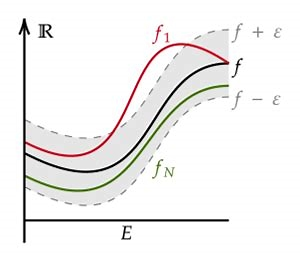
\includegraphics[width=0.5\linewidth]{Images/EpisilonTube.png}
    \caption{Epsilon-Tube}
\end{figure}
\begin{defn}
    We say that $f_n \to f$ \textbf{pointwise} if for all $\epsilon>0,$ for each $x \in X,$ there exists some $N_x \in \bbN$ such that if $n\geq N_x,$ then we have that 
    \[d(f_n(x), f(x))< \epsilon.\]
\end{defn}
You can see now that uniform convergence is strictly stronger than pointwise convergence. The classic theorem to begin with is when do we have continuity of $f?$
\begin{thm}
Suppose $f_n$ is continuous for all $n.$ If $f_n \to f$ unif. then $f$ is continuous.
\end{thm}
\begin{proof}
Let $\epsilon>0$ and $x\in X.$ Since $f_n \to f$ uniformly, we have that there exists some $N \in \bbN$ such that if $n\geq N,$ we have that 
\[d(f_N(x), f(x))< \frac{\epsilon}{3}\qquad \forall x\in X.\] Since $f_N$ is continuous, then there exists some $\delta>0$ such that if $y\in X$ with $d(x,y)< \delta,$ then 
\[d(f_N(x), f_N(y))< \frac{\epsilon}{3}.\] Thus, 
    \[d(f(x),f(y))\leq d(f(x), f_N(x)) + d(f_N(x), f_N(y)) + d(f_N(y))  < \frac{\epsilon}{3} + \frac{\epsilon}{3} + \frac{\epsilon}{3}.\]
\end{proof}
Pointwise convergence is not enough to satisfy continuity as per the following example.
\begin{exmp}
    Let $f_n: [0,1]\to \bbR$ with $f_n = x^n.$ To show that \[\lim_{n\to \infty} f_n = \begin{cases}
        0, \qquad x\in [0,1)\\
        1, \qquad x = 1
    \end{cases},\] consider that if $x\in [0,1),$ then $\lim_{n\to \infty}x^n = 0$ and if $x=1,$ then the limit is simply $1.$ To show that the convergence is not uniform, we must show that the $N$ is dependent on both $\epsilon$ and $x.$ Thus, let $\epsilon = \frac{1}{2},$ then assume there exists some $N$ for uniform convergence. This $N$ will then work for any $x,$ say $x = (\frac{2}{3})^{\frac{1}{N}},$ but then
    \[d(f_N(x), f(x)) = |x^N - 0| = x^N = (\frac{2}{3})^{\frac{1}{N}^N} = \frac{2}{3} >\epsilon.\]
\end{exmp}
\begin{defn}
    We say the \textbf{space of bounded functions} is $C_b$ and the \textbf{space of continuous functions} is $C^0 = C^0([a,b], \bbR).$
\end{defn}
\begin{rem}
    Note that by the EVT, $C^0 \subset C_b.$ Also not that by Theorem 20, if $f$ is a limit point of $C^0,$ then we have a sequence of continuous functions converging (with respect to the sup metric, i.e, uniform convergence) to $f$ implying that $f$ is in fact continuous. Thus, $C^0$ is closed.
    \end{rem}
\begin{thm}
    $C_b$ is complete.
\end{thm}
\begin{proof}
    Let $(f_n)$ be Cauchy in $C_b.$ For any $x$ in the domain, we have that $(f_n(x))$ is a bounded Cauchy sequence in $\bbR,$ and thus must converge. For each $x,$ we let $\lim_{n\to \infty}f_n(x) = f(x).$ We claim that the convergence is also uniform! Let $\epsilon>0.$ By Cauchyness, we have that there exists some $N$ such that if $n,m \geq N,$ we have 
    \[d(f_n, f_m)< \frac{\epsilon}{2}.\] By pointwise convergence, exists some $m\geq N$ dependent on $x$ such that 
    \[d(f_{m(x)}, f(x))< \frac{\epsilon}{2}.\] Thus, we use the $N$ from Cauchy and we know that if $n\geq N,$ we have that:
    \[d(f_n(x), f(x)) \leq d(f_n(x), f_{m(x)}(x)) + d(f_{m(x)}, f(x))< \epsilon.\]
\end{proof}
Note that we are using a different $m$ for each $x$ in this proof, but it doesn't matter at the end of the day because we know that given some $N,$ then for any $x,$ we can find this $m$ by the pointwise convergence.
\begin{cor}
    $C^0$ is complete.
\end{cor}
For this one-liner, use Remark 10 and Theorem 21.\\
What else does uniform convergence imply?
\begin{thm}
    Suppose $f_n \to f$ uniformly with each $f_n$ integrable. Then $f$ is integrable. Moreover, 
    \[\int f_n \to \int f, \quad \text{uniformly}\]
\end{thm}
The spirit of the proof is that we can bound the upper and lower sums of $f$ by upper and lower sums of $f_n.$ Pugh presents a cleaner proof using the Riemann-Lebesgue Integrable Criterion:
\begin{proof}
    Since each $f_n$ is integrable, then each $f_n$ has countably many discontinuities. Call this set $D_n.$ Then each $f_n$ is continuous for any $x\in [a,b]\setminus D_n,$ and thus Theorem 20 states that $f$ must be continuous for any $x\in [a,b]\setminus \bigcup D_n.$ We have that $f$ is bounded by Theorem 21. Thus by the Riemann-Lebesgue Theorem, $f$ is integrable.\\
    Let $\epsilon>0.$ From uniform convergence, there exists some $N$ such that if $n\geq N,$ we have that $d(f_n, f)< \frac{\epsilon}{b-a}$
    
    Get the $N$ from the uniform convergence of $f_n,$ then 
    \[\left|\int_a^x f_n(t)dt  - \int_a^x f(t)dt\right| = \left| \int_a^x (f_n(t) - f(t))dt\right| \leq \int_a^x |f_n(t) - f(x)|dt \leq d(f_n, f)(b-a)< \epsilon.\]
\end{proof}
Luis forgot (didn't care) to mention the Weierstrass-M test, but here it is. It is a useful criteria for deciding when a power series converges. 
\begin{thm}
    (Weierstrass-M test) Let $(f_n)\in C_b.$ Suppose that for each $n,$ $||f_n||\leq M_n,$ where $M_n$ forms a convergent series. Then $\sum |f_n|$ converges uniformly. 
\end{thm}
\begin{proof}
    We use our most powerful theorem, $C_b$ is complete. We must show that the series is Cauchy, or better, that the partial sums, $F_n = \sum_{k=0}^n f_k$ are Cauchy. Suppose $m> n,$ then we have that
    \[d(F_n, F_m) \leq d(F_m, F_{m-1}) + \dots + d(F_{n+1}, F_n) = \sum_{k= n+1}^m ||f_k|| \leq \sum_{k=n+1}^m M_k.\]
\end{proof}
Looking back on this with the foresight of functional analysis, the M-test reminds me a ton of the Banach-Steinhaus Uniform Boundedness Principle (foreshadowing).

\newpage

\subsection{Fri, Oct 25: Arzela-Ascoli}
The second half of the lecture fucks. Persevere!
\begin{thm}
Suppose $f_n$ is differentiable for all $n.$ Suppose $f_n \to f$ uniformly and $f_n'$ converges uniformly. Then $f$ is differentiable and moreover $f_n' \to f'$ uniformly. 
\end{thm}
\begin{proof}
    We weaken the statement and assume $f_n \in C^1$ just to make the proof enjoyable. We apply FTC and Theorem 22. Note that all the following convergenes are uniform.
    \[f_n(x) = f_n(a) + \int_a^x f_n'(t)dt \to f(a) + \int_a^x g(t)dt \implies f'(x) =  g(x).\] We leave the proof of the actual statement to the gods.
\end{proof}
We can now use the Weirstrass-M test!
\begin{prop}
    A power series converges uniformly on $[-r,r],$ where $|r|< R$ is the radius of convergence.
\end{prop}
\begin{proof}
    Let $\sum c_k x^k$ be a power series. We have that for large  $k,$ $ \frac{1}{\sqrt[k]{c_k}}< \beta <R,$ and thus we have that for large $k:$
    \[x^kc_k \leq \left(\frac{x}{\beta}\right)^{k},\] where the right side forms a geometric power series. Thus, we have our result by Weirstrass-M.
\end{proof}
Now we get to the good stuff. First, a definition.
\begin{defn}
    Let $\mathcal{E}$ be a family of functions. We say $\mathcal{E}$ is equicontinuous if for  any $\epsilon>0,$ there exists some $\delta>0$ such that if $d(x,y)< \delta$ and $f\in \mathcal{E},$ then \[d(f(x), f(y)) < \epsilon.\]
\end{defn}
To make sense of this definition, think of it as uniform continuity of a bunch of functions. There is some $\delta$ that determines the continuity of every function in the family.
\begin{exmp}
    Suppose $f_\alpha: [a,b]\to \bbR$ and $||f_{\alpha}||< A$ for any $\alpha.$ Then we have by the MVT that if $\alpha \in \mathcal{A}$ and $x,y \in [a,b]$ then
    \[|f_\alpha(x)- f_\alpha(y)| \leq |f'(\lambda)||x-y|\leq A|x-y|.\] Thus, the family is equicontinuous since they are governed by a \textbf{modulus of continuity}. 
\end{exmp}
Here is a very very important theorem with a very very cool name.
\begin{thm}
    (Arzela-Ascoli) Any bounded equicontinuous sequence of functions in $C^0([a,b], \bbR)$ has a uniformly convergent subsequence.
\end{thm}
\begin{proof}
Since $[a,b]$ is compact, there exists some countably dense subset $D \subset [a,b]$ (exercise). Let $D = \{d_1, d_2, \dots\}.$ Consider that $(f_n(d_1))$ forms a bounded sequence of reals, and thus by Bolzano-Weierstrass must have a convergent subsequence $(f_{n, 1}(x))$ which converges at $d_1.$ Consider that $(f_{n, 1})(d_2)$ forms a bounded sequences of reals, and must have a convergent subsequence $(f_{n,2}(x))$ which converges at $d_2.$ However, since this subsequence is a subsequence of a sequence which converges at $d_1,$ then it also converges at $d_1.$ Keep going in this way, then consider the sequence $(f_{i,i})(x).$ That is, we are consider the following diagonal sequence:
\[
\begin{array}{ccccccc}
f_{1,1}(x) & f_{2,1}(x)& f_{3,1}(x) & f_{4,1}(x) & f_{5,1}(x) & \cdots \\
         & f_{2,2}(x) & f_{3,2}(x) & f_{4,2}(x) & f_{5,2}(x) & \cdots \\
         &          & f_{3,3}(x) & f_{4,3}(x) & f_{5,3}(x) & \cdots \\
         &          &          & f_{4,4}(x) & f_{5,4}(x) & \cdots \\
         &          &          &          & f_{5,5}(x) & \cdots \\
         &          &          &          &          & \ddots \\
\end{array}
\]
For any $d_k \in D,$ $f_{i,i}(x)$ converges at $d_k.$ Thus, we have that for any $d_k,$ there exists some large $N$ such that if $i, j \geq N,$ we have that 
\[d(f_{i,i}(d_k), f_{j,j}(d_k))< \frac{\epsilon}{3}.\] We have that each $f_{i,i}$ is continuous on a compact set (and thus uniformly continuous), and so there exists some $\delta>0$ such that if 
\[d(x,y)< \delta \implies d(f_{i,i}(x), f_{i,i}(y))< \frac{\epsilon}{3}.\] For any $x\in [a,b],$ there exists some $d_k \in D$ such that $d(x, d_k)< \delta.$ Thus, for any $\epsilon>0,$ there exists this $\delta$ such that if $x,y \in [a,b],$ then 
\[d(f_{i,i}(x), f_{j,j}(x))\leq d(f_{i,i}(x), f_{i,i}(d_k)) + d(f_{i,i}(d_k), f_{j,j}(d_k)) + d(f_{j,j}(d_k), f_{j,j}(y))\leq \frac{\epsilon}{3} + \frac{\epsilon}{3} + \frac{\epsilon}{3}.\] Again, the first and last distances in the inequality above are bounded due to uniform continuity of the individual $f_n,$ and the middle one is bounded from equicontinuity.\\

We have that $(f_{i,i})$ is Cauchy, and thus converges  since $C^0$ is complete.
\end{proof}
This theorem has countless consequences, but the most important is the following.
\begin{thm}
    (Heine-Borel) $\mathcal{E}\subset C^0$ is compact if and only if it is equicontinuous, closed, and bounded.
\end{thm}
\begin{proof}
    We prove both directions.
    \begin{itemize}
        \item ($\implies$) Suppose $\mathcal{E}$ is compact. Closed and bounded are immediate. We can find a finite $\epsilon-3$ dense subset of $\mathcal{E}$ by compactness (exercise). Let $\{f_{k_\frac{\epsilon}{3}} \; : \; k \in [n]\}$ be such a subset. Thus, if $f\in \mathcal{E},$ then there exists some $f_k$ such that $d(f, f_k)< \frac{\epsilon}{3}.$ Suppose $x,y \in [a,b]$ and $d(x,y)<\delta,$ where $\delta$ is the one from uniform continuity, then 
        \[d(f(x), f(y))\leq d(f(x), f_k(x)) + d(f_k(x), f_k(y)) + d(f_k(y), f(y))< \frac{\epsilon}{3} + \frac{\epsilon}{3} + \frac{\epsilon}{3}.\] Again, the middle distance is bounded by uniform continuity, and outer ones by the dense subset.
        \item ($\impliedby$) Let $(f_n)\in \mathcal{E}.$ By equicontinuity and boundedness, Arzela-Ascoli tells us that we have a convergent subsequence $(f_{n_k})$ and closedeness tells us the limit lies within $\mathcal{E}.$
    \end{itemize}
\end{proof}
\begin{rem}
    $f_n$ converges uniformly if and only if $f_n$ are equicontinuous and converge pointwise.
\end{rem}
The proof of the remark is an $\epsilon /3$ mess, but try it out. 

\newpage
\subsection{Mon, Oct 28: Weierstrass Approximation Theorem}
We discuss convolutions and the Weierstrass Approximation Theorem. It is a cool result with an unfortunately not cool (in my opinion) proof.
\begin{defn}
    A \textbf{convolution} is defined by \[f \ast g = \int_\bbR f(x-y)g(y)dr = \int_\bbR g(x-y)f(y)dy.\]
\end{defn}
\begin{rem}
    Suppose $f \in C^1$ and $g$ have support (set where $g$ outputs nonzero values) on $[a,b].$ Then \[(f\ast g)'(x) = \lim_{h\to 0}\frac{1}{h}\int f(x + h -y)g(y)dy - \int f(x-y)g(y)dy = \int f'(x-y)g(y)dy = (f' \ast g)(x)\]
\end{rem}
\begin{prop}
    The convolution of a not smooth function can be made smooth.
\end{prop}
I apologize for this, Luis was pretty bad with it and I don't care enough about convolutions to fix his lecture.
\begin{proof}
    Let $f: [a,b]\to \bbR$ be smooth with $f(a) = f(b) = 0$ with support on $(a,b).$ Let $(g_n)$ such that $g_n$ has support on $[-\frac{1}{n}, \frac{1}{n}]$ and $\int_\bbR g_n(y)dy = 1.$ Then 
    \begin{align*}
        |(f\ast g_n)(x) - f(x)| &= \int_\bbR |f(x-y) - f(x)| - g_n(y)dy\\
        &= \int_{-\delta}^\delta f(x-y) - f(x)g_n(y)dy + \int_{\bbR \setminus [-\delta, \delta]}|f(x-y) - f(x)| g_n(y)dy\\
        &\leq \epsilon + C\int_{\bbR \setminus [-\delta, \delta]} g_n dy \to 0.
    \end{align*}
\end{proof}
\begin{thm}
    (Weirstrass Approximation Theorem) Polynomials are dense in $C^0([a,b], \bbR).$ 
\end{thm}
The proof follows from the above and also the fact that if $P$ is a polynomial, then $f \ast P$ is a polynomial.

\newpage
\subsection{Wed, Oct 30: Banach Contraction Principle and Picard's Theorem for ODEs}
This lecture is awesome sauce, so strap in. 
\begin{defn}
    We say $f: M \to M$ is a \textbf{contraction} if there exists some $k<1$ such that for any $x,y \in M:$
    \[d(f(x), f(y))\leq kd(x,y).\]
\end{defn}
\begin{defn}
    We say $f$ has a \textbf{fixed point} at some $x$ if $f(x) = x.$
\end{defn}
\begin{thm}
    (Brouwer) Suppose $f: B_1(0) \to B_1(0)$ is continuous, then $f$ has a fixed point.
\end{thm}
The proof for this will hopefully be on the last page of this document. We turn to another fixed-point theorem, which has an awesome proof.
\begin{thm}
    (Banach) Suppose that $M$ is complete and $f:M \to M$ is a contraction. Then $f$ has a fixed point.
\end{thm}
The idea for this proof is that eventually enough contraction results in a single point.
\begin{proof}
    Let $x_0 \in M.$ Let $x_1 = f(x_0),$ $x_2 = f(f(x_0)),$ and $x_n = f^{(n)}(x_0).$ We wish to show that $(x_n)$ is Cauchy. Consider that for any $n:$
    \[d(x_{n}, x_{n+1}) = d(f(x_{n-1}, f(x_n))\leq k d(x_{n-1}, x_n) \leq k^{n}d(x_0, x_1).\] Thus, if $n>m,$ we have that 
    \[d(x_n, x_m) \leq d(x_n, x_{n+1}) + d(x_{n+1}, d_{n+2}) + d(x_{m-1}, x_m) \leq k^{n}d(x_0, x_1) + k^{n+1}d(x_0, x_1) + \dots k^{m-1}d(x_0, x_1) = d(x_0, x_1)(\frac{k^n}{1-k}).\] Since $k<1,$ we have that as $n\to \infty,$ $d(x_n, x_m)\to 0,$ and thus $(x_n)$ is Cauchy, and by the completeness of $M,$ we have $(x_n)\to x_\infty \in M.$ We claim that $f(x_\infty) = x_\infty.$ That is, $x_\infty$ is our fixed point. To show this, consider that 
    \[d(f(x_\infty), x_\infty) \leq d(f(x_\infty), f(x_n)) + d(f(x_n), x_n) + d(x_n, x_\infty)\leq kd(x_\infty, x_n) + kd(x_\infty, x_n) + k^{n-1}(x_0, x_1) + d(x_\infty, x_n)\to 0.\]
\end{proof}
How can we guarantee the existence and uniqueness for a solution of an ODE?
\begin{thm}
    (Picard) Suppose $F: \Omega \to \bbR^d$ with $\Omega$ open is Lipshitz. Suppose $x_0 \in \Omega,$ then there exists some unique trajectory $\gamma: (a,b)\to \Omega$ that if $\gamma(0) = x_0,$ then $\gamma'(t) = F(\gamma(t)).$
\end{thm}
\begin{proof}
    Solving the ODE in the problem statement is equivalent to finding the solution to 
    \[\gamma(t) = x_0 + \int_0^t F(\gamma(s))ds.\]
    We can only find this solution locally, so restrict $F$ to some compact $\overline{B_r(x_0)}.$ By continuity of $F,$ we have that $F$ is locally bounded here by some $M.$ Choose $\tau$ small such that 
    \[\tau M \leq r, \qquad \tau L <1.\]
    Define $\m: \mathcal{M}\to \bbR,$ where 
    \[\mathcal{M} = \{f: [-\tau, \tau] \to \Omega\; : \; \text{$f$ is continuous}\}.\] With respect to $d_{sup},$ $\mathcal{M}$ is complete. Define $m$ by 
    \[m(\gamma(t)) = p + \int_0^t F(\gamma(s))ds.\] By Banach's Contraction principle, it suffices to show that $m$ is a contraction and it maps functions to $\mathcal{M}$. Let $\sigma, \gamma \in \mathcal{M},$ then we have that 
    \[d(m(\sigma), m(\gamma)) = \sup_{t}\left|\int_0^t F(\gamma(s)) - F(\sigma(s))ds\right|\leq \tau \sup_{t}|F(\gamma(t)) - F(\sigma(t))|\leq \tau Ld(\gamma(t), d(\sigma(t))).\] Since $\tau L <1,$ we have that $m$ is a contraction. Suppose $\gamma \in \mathcal{M}.$ Then we have that 
    \[m(\gamma(t)) = x_0 + \int_0^t F(\gamma(s))ds\leq x_0 + \tau M \implies d(x_0, m(\gamma(t))) \leq r \implies m(\gamma)\in \overline{B_r(x_0)}.\] Thus, we have the existence of some $\gamma$ that satisfies the conditions.
\end{proof}
Suppose we have a river $(\Omega)$ and some rock thrown at some point in the river $(x_0\in \Omega).$ Picard guarantees us that if the velocity/flow of the river is Lipshitz, then we can put some boat where the rock landed who's path ($\gamma(t)$) will move in the flow of the river in some time interval $t\in [-\tau, \tau]$.  
\begin{exmp}
    Suppose $f(x) = x^2.$ Then $f$ is not global Lipshitz, and so we have the consequence that the solution blows up in local time. I.e, we can find a solution in local but not global time:
    \[\gamma'(t) = (\gamma(t))^2 \implies \gamma(t) = \frac{1}{2-t},\] which blows up near $x = 2.$ 
\end{exmp}

\begin{exmp}
Suppose $f(x) = \sqrt{x},$ thn $\gamma(t) = 0$ or $\gamma(t) = \frac{1}{4}t^2.$ However, since we do not have Lipshitz, we also have that 
\[\gamma(t) = \begin{cases}
    \frac{(x-a)^2}{4}, \quad x >a\\
    0, \qquad x<0
\end{cases}\]
and so our solution is not unique!
\end{exmp}

\newpage
\subsection{Fri, Nov 1: Baire Category Theorem and Consequences}
The best theorem of all time. If I were a lemma I would go out with Baire Category Theorem, even though I hardly know him!
\begin{thm}
    Let $(G_n)$ be a countable collection of open dense sets in $M,$ a complete metric space. Then 
    \[\bigcap G_n\] is dense in $M.$
\end{thm}
\begin{proof}
    Let $p \in M$ and $\epsilon>0.$ Since $B_\epsilon(p_0)$ is open, then there exists some $r_0>0$ and $p_1 \in M$ such that
    \[\overline{B_{r_0}(p_1)}\subset B_\epsilon(p_0).\] Since $G_1$ is open, there exists some $r_1>0$ and $p_2 \in M$ such that 
    \[\overline{B_{r_1}(p_2)}\subset B_{\frac{r_0}{2}}\cap G_1,\] where the intersection is nonempty by the density of $G_1.$ Make the sequence $(p_n)$ such that
    \[\overline{B_{r_{n-1}}(p_n)} \subset B_{\frac{r_{n-2}}{2}}\cap G_1 \cap G_2 \cdots \cap G_{n-1}\] We have that $r_n \to 0$ since $r_{n+1}\leq \frac{r}{2}$ and so 
    \[\lim_{n\to \infty}\text{diam}\overline{B_{\frac{r}{2}}(p_n)}\to 0,\] implying that $(p_n)$ is Cauchy. Moreover, we have that each $(p_n)\in B_\epsilon(p_0).$ Since $M$ is complete, we have that $(p_n)\to p_\infty\in M,$ and we must also have that $p_\infty \in B_\epsilon(p_0)$ and also that for each $n,$ $p_\infty \in G_n.$ Thus, for any $p_0 \in M,$ and $\epsilon>0,$ there exists some $p_\infty \in M$ such that 
    \[p_\infty \in B_\epsilon(p_0)\cap \bigcap G_n,\] implying that the intersection is dense in $M.$ 
\end{proof}
\begin{cor}
    Suppose $M$ is complete and 
    \[M = \bigcap F_n\] where each $F_n$ is closed. Then at least one $F_i$ must have some nonempty interior.
\end{cor}
\begin{proof}
    Suppose not. That is, suppose we can write 
    \[M = \bigcup F_n\] where $F_n$ closed has an empty interior for any $n.$ Thus, we have that 
    \[\emptyset = M^c = (\bigcup F_n)^c= \bigcap F_n^c\] is an intersection of open dense sets (the compliment of empty interior is a dense set). Thus, we have by Baire's theorem that $\emptyset$ must be dense in $M.$ Ridiculous! 
\end{proof}
Baire Category Theorem allows us to prove some pretty insane stuff. Luis of course didn't prove them, but they are still cool!
\begin{thm}
    The set of continuous and nowhere-differentiable functions is general in $C^0.$ That is, this set is dense in $C^0.$
\end{thm}
Sketch: define
\[G_n := \{f \in C^0([a,b], \bbR)\; : \; \forall x\in [a, b-\frac{1}{n}], \exists y>x \; s.t. |f(y)-f(x)|\geq n|x-y|\}.\] We claim that $G_n$ is open and that $G_n$ is dense in $C^0.$ 

\subsection{Mon, Nov 4: The Derivative in Higher Dimensions}
So get ready for the worst thing in analysis.
In $1-D,$ we defined the derivative of a function $f: \bbR \to \bbR$ to be the limit
\[\lim_{h\to 0}\frac{f(x+h) - f(x)}{h} = f'(x)\iff f(x+h) = f'(x)h +f(x),\] where we take the right hand in the limit as $h\to 0.$
\begin{defn}
    The \textbf{total derivative} of $f: \bbR^n \to \bbR^m$ at $x\in \bbR^n$ if it exists, is the limit linear transform $Df_x$ such that
    \[f(x+h) = f(x) + Df_x  + R(h), \quad \lim_{|h|\to 0}\frac{|R(h)|}{|h|}\to 0,\] where $||$ is the vector norm and $R(h)$ is an error term.
\end{defn}
Since $Df_x$ is a linear operator, it will be useful to talk about some linear algebra. In particular, lets define the stretch a linear transform $T$ applies to vectors.
\begin{defn}
    Suppose $T: V \to W$ is a linear transformation, we define the \textbf{operator norm} of $T$ to be 
    \[||T|| = \sup_{v\in V}\frac{|T(v)|_W}{|v|_V},\] where $|\cdot|_W$ and $|\cdot|_V$ are the norms of vectors in $V$ and $W.$
\end{defn}
You might have seen it with different definitions, we remark that this is equivalent to saying that 
\[||T|| = \sup_{v\in V}|T(v)|.\] In particular, we have the following theorem:
\begin{thm}
    The following are equivalent:
    \begin{enumerate}
        \item $||T||$ is finite.
        \item $T$ is uniformly continuous.
        \item $T$ is continuous at the origin (or any point in $V$ for that matter).
    \end{enumerate}
    \end{thm}
\begin{proof}
    Let $\epsilon>0.$ There exists a $\delta = \frac{\epsilon}{||T||}$ such that if $v, v' \in V$ with $|v - v'|< \delta,$ then 
    \[|T(v) - T(v')| = |T(v - v')| \leq ||T|||v-v'.|\] Two obviously proves three. Suppose $T$ is continuous at $0.$ Let $v \in V.$ Then let $\epsilon = 1,$ and so we have that that for any $\delta>0,$ if $|u|< \delta,$ then
    \[|T(u)| \leq 1.\] Thus, if we let $u = \frac{\delta v}{2|v|},$ then 
    \[\frac{|T(v)|}{|v|} = \frac{T(u)}{|u|}\leq \frac{2}{\delta}< \infty.\]
\end{proof}
Moreover, we have the following theorem:
\begin{thm}
    Suppose $W$ is a finite dimensional vector space, then any linear transform $T: \bbR^n \to W$ is continuous. In fact, if it is an isomorphism then it is a homeomorphism.
\end{thm}
\begin{defn}
    We define the \textbf{partial derivative} of $f_j: \bbR^n \to \bbR$ at $x$ to be 
    \[(Df_j)_x(e_i) = D_if_j(x) = \partial_i f_j(x) =\frac{\partial f_j}{\partial x_i}(x) = \lim_{|h|\to 0}\frac{f_j(x_1, x_2, \dots, x_i + h, \dots, x_n) - f_j(x)}{|h|} = \lim_{|h|\to 0}\frac{f_j(p + te_i) - f_j(p)}{|h|}.\]
\end{defn}
\begin{rem}
    In high school calculus textbooks, the total derivative of $f$ at $x$ would be denoted by the $m\times n$ matrix of partials:
    \[Df_x = \begin{bmatrix}
        D_1f_1 & D_2f_1 & \cdots & D_nf_1\\
        D_1f_2 & D_2f_2 & \cdots & D_nf_2\\
        \vdots & \vdots & \ddots & \vdots\\
        D_1f_m & D_2f_m & \cdots & D_nf_m
    \end{bmatrix}.\]
\end{rem}
    \begin{thm}
        If every $\partial_i f_j(x)$ exists and is continuous for all $i\in [n]$ and $j \in [m],$ then $f$ is differentiable. 
    \end{thm}
This proof is severely unenjoyable and I refuse to type it up for now.
\begin{prop}
    The total derivative satisfies the following properties:
    \begin{enumerate}
        \item $D(f + g) = Df + Dg$
        \item $D(f\circ g) = Df \circ Dg$
        \item $D(f\cdot g) = Df \cdot g  + f\cdot Dg$ (where $\cdot$ is the dot product).
    \end{enumerate}
\end{prop}
We give the best possible version of the Mean Value Theorem we can.
\begin{thm}
    Suppose $f: \bbR^n \to \bbR^m$ is differentiable on $U$ and $[p,q]\subset U,$ then 
    \[|f(q) - f(p)|\leq \sup_{x\in U}Df_x|q-p|.\]
\end{thm}
\begin{proof}
    Let $u\in \bbR^n$ be the unit vector, then if $t\in [0,1],$ we get that
    \[g(t) = \langle u, f(p + t(q-p))\rangle\] is differentiable and real valued, and thus we use the 1-D MVT to get some $\theta \in [0,1]$ such that 
    \[g(1) - g(0) = \langle u, f(q) - f(p)\rangle = g'(\theta)\]
    and using Proposition 11, we get that 
    \[g'(\theta) = \langle u, Df_{p + \theta(q-p)}(q-p)\rangle \leq \sup_{x\in U}Df_x|q-p|.\] Thus, we have that it has norm less than the desired quantity.
\end{proof}

We have that $Df$ is a linear transform $T: \bbR^n \to \bbR^m.$ The second derivative $D^2f$ is a function $D^2f: \bbR^n \to L(\bbR^n, \bbR^m),$ where $L$ is the space of linear transforms like $T.$ Thus,$v,w$ can take in two vectors $D^2(v)(w)$ and output a vector in $\bbR^m.$
\begin{thm}
    If $f: U \to \bbR^m$ is $C^1$ and if the segment $[p,q]\subset U,$ then 
    \[f(q) - f(p) = T(q-p),\] where $T$ is the average derivative
    \[T = \int_0^1(Df)_{p + t(q-p)}dt.\]
\end{thm}
\begin{defn}
    Assume $f: \bbR^n \to \bbR$ is second differentiable, then we say that $D^2f_x$ is the \textbf{Hessian} of $f.$ That is, the matrix of second partial derivatives.
\end{defn}
\begin{thm}
    The Hessian is symmetric. That is, for any $v, w \in \bbR^n$ we have that 
    \[(D^2f)_x(v)(w) = (D^2f)_p(w)(v).\]
\end{thm}
\begin{rem}
    This does imply that partial double derivative are symmetric since 
    \[(D^2f_x)(e_i)(e_j) = \frac{\partial f_k}{\partial x_i \partial x_j} = \frac{\partial f_k}{\partial x_j x_i} = (D^2)_x(e_j)(e_i)\]
\end{rem}
Have fun proving this one.
    
\newpage
\subsection{Wed, Nov 6: $C^r$ Space}
\begin{defn}
    We say $f\in C^r(U, \bbR^m)$ if the $r$th derivative of $f$ exists and is continuous. 
\end{defn}
\begin{defn}
    The $C^r$ norm of a function $f\in C^r$ is defined by 
    \[||f||_{C^r} = \max\{\sup_{x\in U}|f(x)|, \dots, \sup_{x\in U}|D^{(r)}(x)|\}.\]
\end{defn}
\begin{defn}
    We say that a series $f_k$ is \textbf{$C^r$ uniformly convergent} to some $f$ ($f_k \to f$ $C^r$ unif) if
    \[f_k \to f \quad \text{unif.}\]
    \[(Df_k) \to Df \quad \text{unif}\]
    \[\vdots\]
    \[(D^{(r)}f_k) \to D^{(r)}f \quad \text{unif}\]
\end{defn}
\begin{defn}
We say that a series $f_k$ is $C^r$ \textbf{Cauchy} if for all $\epsilon>0,$ there exits some $N \in \bbN$ such that if $k, \ell >N,$ then
\[||f_k - f_{\ell}||< \epsilon\]
\[||(Df_k) - Df_{\ell}||< \epsilon\]
\[\vdots\]
\[||(D^{(r)}f_k) - (D^{(r)}f_\ell)||< \epsilon\]
\end{defn}
\begin{thm}
    $C^r$ is a \textbf{Banach Space,} i.e, a complete normed vector space. 
\end{thm}
\begin{proof}
    Let $f_k$ be $C^r$ Cauchy. Since $C^0$ is complete, we have that $f_k \to f$ uniformly. We also know that $(Df_k)\to G$ uniformly. We claim that $(Df_k)\to (Df)$ uniformly (i.e, $(Df_k) = G$). Let $p \in U$ and consider $q\in U$ such that $[p,q]\subset U.$ By Theorem 37, we have that 
    \[f_k(q) - f_k(p) = \int_0^1(Df_k)_{p + t(q-p)}dt (q-p)\to f(q) - f(p) = \int_0^1 G(p + t(q-p))dt (q-p).\] Proceed by induction.
\end{proof}

\newpage

\subsection{Fri, Nov 8: The Inverse and Implicit Function Theorem} Both Pugh and Luis have godawful explanations for this. I defer to the Youtube Channel ``The Bright Side of Mathematics."
\begin{thm}
    Let $U, V \subset \bbR^n$ and $f\in C^1(U,V)$ and $x_0 \in U.$ If $(Df)_{x_0}$ is invertible, then $f$ is a local $C^1$ diffeomorphism at $x_0.$
\end{thm}
\begin{proof}
    (STEP 1) If $y_0 = f(x_0),$ then define $\hat{f} = f - y_0$ and define $g(x) = \hat{f}(x + x_0).$ Thus, we have that $\hat{f}(0) = 0$and $(Df)_0$ is invertible. Define $h(x) = (Df)_0^{-1}g(x),$ then $(Dh)_0 = \textbf{I}.$\\

    (STEP 2) Now that we have normalized the problem, we can begin. Let $z(x) = h(x) - x,$ then $(Dz)_0 = \textbf{0}.$ Since $z\in C^1,$  then by continuouity we choose $\epsilon>0$ such that 
    \[\left|\frac{\partial f_i(x)}{\partial x_j}\right|\leq \frac{1}{2}\frac{1}{n^2}, \qquad \forall i, j \in [n], \quad \forall x\in \overline{B_\epsilon(0)}\] and $(D_h)(x)$ is invertible for all $x \in B_\epsilon(0).$\\

    (STEP 3) Now that we have restricted our function to a convex ball, we can use the Mean Value Theorem when we define $a: [0,1]\to \bbR$ by 
    \[a(t) = z_i(p + t(q-p)),\] where $p,q \in B_\epsilon(0).$ Thus, we have that if 
    \[z(q) - z(p) = a(1) - a(0) = a'(\theta) = \langle\nabla z_i(p + \theta(q-p)), p-q\rangle.\] Thus, we have by Cauchy-Schwartz that 
    \[|z(q) - z(p)| \leq ||\nabla z_i(p + \theta(q-p))||^2||p-q||^2 =  \sum_{j}\left|\frac{\partial z_i}{\partial x_j}\right|^2 ||q-p||^2\leq \frac{1}{4}\frac{n}{n^4}||q-p||\] Thus, we have that 
    \[||z(q) - z(p)||^2  = \sum_{i}|z_i(q) - z_i(p)|^2 \leq \frac{1}{16}\frac{1}{n^2}||p-q||^2,\] thus, $z$ is a contraction since
    \[||z(q) - z(p)||| \leq \frac{1}{2}||q-p||.\]

    (STEP 4) Fix an element $y \in \overline{B_\epsilon(0)}$ and define $z_y: \overline{B_\epsilon(0)} \to \overline{B_\epsilon(0)}$ by 
    \[z_y(x) = y - z(x).\] Thus, we have that 
    \[||z_y(q) - z_y(p)||\leq \frac{1}{2}||q-p||,\] and by Banach's fixed point theorem, there exists some unique fixed point $x$ such that 
    \[z_y(x) = x \iff y- z(x) = x \iff y - (h(x) - x) = x \iff y = h(x).\] Thus, we have found a bijection in this closed $\epsilon$ ball.\\

    The rest of the proof is left up to the reader.
\end{proof} 
\begin{rem}
    We have a nice formula for the inverse, that being 
    \[(D{h^{-1}})_y = \left((Dh)_{h^{-1}(y)}\right)^{-1}\]
\end{rem}
\begin{thm}
    Suppose $U \subset \bbR^n \times \bbR^m$ is open, and $F: U \to \bbR^m$ is $C^1.$ Let $z_0 = (x_0, y_0)\in U$ with $F(z_0) = 0$ and 
    \[DF_{z_0} = 
    \begin{bmatrix}
        \frac{\partial F_1(z_0)}{\partial x_1} & \frac{\partial F_1(z_0)}{\partial x_2}& \cdots & \frac{\partial F_1(z_0)}{\partial x_n} & \frac{\partial F_1(z_0)}{\partial x_{n+1} & \cdots &\frac{\partial F_1(z_0)}{\partial x_m}}\\
        \frac{\partial F_1(z_0)}{\partial x_1} & \frac{\partial F_2(z_0)}{\partial x_2}& \cdots & \frac{\partial F_2(z_0)}{\partial x_n} & \frac{\partial F_2(z_0)}{\partial x_{n+1} & \cdots &\frac{\partial F_2(z_0)}{\partial x_m}}\\
        \vdots & \vdots & \ddots & \vdots & \vdots & \ddots &\vdots\\
        \frac{\partial F_m(z_0)}{\partial x_1} & \frac{\partial F_m(z_0)}{\partial x_2}& \cdots & \frac{\partial F_m(z_0)}{\partial x_n} & \frac{\partial F_m(z_0)}{\partial x_{n+1} & \cdots& \frac{\partial F_m(z_0)}{\partial x_m}}
    \end{bmatrix}
     = \begin{bmatrix}
         \frac{\partial F}{\partial x} & \frac{\partial F}{\partial y}
     \end{bmatrix}.\] If $\frac{\partial F}{\partial y} \neq \textbf{0},$ then there exists open $V_1 \subset \bbR^n$ and $V_2 \subset \bbR^m$ such that $z_0 \in V_1 \times V_2$ and a map $g\in C^1(V_1,V_2)$ such that 
     \[g(x, g(x)) = 0.\]
\end{thm}
\begin{proof}
    Define $f: U \to \bbR^n \times \bbR^m$ by $f(x,y) = \begin{pmatrix}
        x\\ f(x,y)
    \end{pmatrix}.$ Thus $f\in C^1(U, \bbR^n \times \bbR^m)$ and 
    \[Df_{z_0} = \begin{bmatrix}
        \textbf{I} & \textbf{0}\\
        \frac{\partial F(z_0)}{\partial x} & \frac{\partial F(z_0)}{dy}
    \end{bmatrix}\]
    Thus, we have that $\det Df_{z_0} = 1 \cdot \det DF_{z_0}\neq 0.$ We can apply the inverse function theorem to $f.$ We get open set $U;, V' \subset \bbR^n$ and $f^{-1}: V' \to U'$ is $C^1$ and $f(z_0) = \begin{pmatrix}
        x_0 \\ 0
    \end{pmatrix}  \in R = V_1' \times V_2' \subset V'.$  Let $S = f^{-1}(R),$ we know it is open and $z_0 \in S = V_1 \times _2.$ Thus, $f^{-1}: V_1 \times V_2 \to V_1 \times V_2$ with
    \[\begin{pmatrix}
        x\\y'
    \end{pmatrix} \to \begin{pmatrix}
        x\\ h(x,y')
    \end{pmatrix}\], where \[h: V_1 \times V_2' \to V_2\] is $C^1.$ Thus, define $g: V_1 \to V_2$ such that $g(x) = h(x,0) \in C^1.$ 
\end{proof}


\newpage
\subsection{Mon, Nov 11: Lagrange Multipliers}
\begin{thm}
    Suppose $f: \bbR^n \to \bbR$ and $g_j: \bbR^n \to \bbR$ is $C^1$ for $j \in [m]$ (i.e, $g: \bbR^n \to \bbR^m$). Suppose $f$ has a local extremum at $x_0$ with the constraint $g(x) =0$ and $\text{rank}(Dg_{x_0}) = m.$ Then there are real numbers, called \textbf{Lagrange Multipliers} $\lambda_j \in \bbR$ such that 
    \[\nabla f(x_0) = \sum_{j=1}^m \lambda_j \nabla g_j(x_0)\]
\end{thm}
We will prove this for the $m = 1,$ $n=2$ case, which states that if $f: \bbR^2 \to \bbR$ and $g: \bbR^2 \to \bbR$ is $C^1,$ then if $f$ has a local extremum at $x_0$ with the constraint of $g(x) = 0,$ and $\nabla g(x_0) \neq 0,$ then there exists some $\lambda \in \bbR$ such that 
\[\nabla f(x_0) = \lambda \nabla g(x_0).\]
\begin{proof}
    By the implicit function theorem, we have that $g(x_1, x_2) = 0$ can locally be written as either 
    \[g(x_1, \gamma(x_2)) =0, \qquad \text{or}\qquad g(\beta(x_2), x_2) = 0.\] Let's concentrate on the first. Then for all $x_1 \in U,$ we write $g(x_1, \gamma(x_2)) = 0.$ By assumption, we have that that by the chain rule
    \begin{align}
        0 = \frac{d}{dx_1}g(x_1, \gamma(x_1)) = \langle 
    \nabla g(x_1, \gamma(x_1)), \begin{pmatrix}
        1 \\ \gamma'(x)
    \end{pmatrix}
    \rangle.
    \end{align} We have that the function $\hat{f}: U \to \bbR$ with $\hat{f}(x_1) = f(x_1, \gamma(x_1))$ has a local extremum at $x_{0_1}.$ Thus, we have that 
    \[0 = \hat{f}'(x_{0_{1}}) = \langle \nabla f(x_{0_1}, \gamma(x_{0_1})), \begin{pmatrix}
        1 \\ \gamma'(x_{0_1})
    \end{pmatrix}\rangle\] Because (1) holds for any $x\in U,$ then we have the $\nabla f$ and $\nabla g$ are orthagonal to each other, and so there must exist some real $\lambda$ such that 
    \[\nabla f = \lambda \nabla g.\]
\end{proof}
You can see that the method of Lagrange Multipliers is an application of the implicit function theorem.

\newpage
\subsection{Wed, Nov 13: Multivariate Integration}
We mostly talked about integration from $\bbR^2 \to \bbR.$ 
\begin{defn}
    Suppose $R\subset \bbR \times \bbR$ is a rectangular region. Then we partition $R$ into $R_{i,j} = [x_{i-1}, x_i) \times [y_{j-1}, y_j)$ such that $R = \bigcup_j\bigcup_i R_{i,j}.$ Then we take a sampling of points $S$ inside each $R_{i,j}$ and we call the Riemann Sum to be 
    \[R(f,P,S) = \sum f(s_{i,j})|R_{i,j}| = \sum f(s_{i,j})(x_i - x_{i-1})(y_{i} - y_{i-1}).\]
    We say $f$ is \textbf{Riemann Integrable} if there exists some $I \in \bbR$ such that for all $\epsilon>0,$ there exists some partition $P$ such that 
    \[|P-I|< \epsilon.\]
\end{defn}
\begin{defn}
    We define the \textbf{upper sum} and the \textbf{lower sum} to be 
    \[U(f,P) = \sum \max f |R_{i,j}|, \qquad L(f,P) = \sum \min f |R_{i,j}|.\] We say that $f$ is\textbf{Darboux integrable} if for any $\epsilon>0,$ there exists partitions $P$ such that 
    \[|U(f,P) - L(f,P)| < \epsilon \iff \inf U = \sup L.\]
\end{defn}
\begin{rem}
    Notationally, we say that \[\underline{\int}fdxdy = \sup L, \qquad \overline{\int}f dxdy = \inf U\]
\end{rem}
Sliced Bread.
\begin{thm}
    (Fubini's Theorem) If $f$ is integrable over $R = [a,b] \times [c,d],$ then 
    \[\int_R fdxdy = \int_c^d \left[\int_a^b f dx \right]dy.\]
\end{thm}
\begin{proof}
    \[U = \inf\{\int_R g dxdy; \; g\geq f, \quad \text{$g$ constant on $R_{i,j}$}\}\]
    \[L = \sup\{\int_R g dxdy;\;  g\leq f, \quad \text{$g$ constant on $R_{i,j}$}\}\]
Thus, 
\[\int_c^d \left[\int_a^b gdx\right]dy = \sum g(s_{i,j})|R_{i,j}|.\]
For any $g$ with $g\leq f$ we have
\[\underline{\int_c^d}\left[\underline{\int_a^b}fdx\right]dy \geq \underline{\int_c^d} \underline{\int_a^b} gdxdy = \int_R g dxdy \leq \int_R f dxdy\]
and thus 
\[\]
\end{proof}

We now pivot to a very important theorem in multidimensional calculus: 
\begin{thm} (Inverse Function Theorem)
    Suppose $\varphi: U \to W$ is a $C^1$ differeomrphism with $U,W$ open. Suppose further that $f$ is integrable and that $R \subset U.$ Then we have that 
    \[\int_{\varphi(R)}f = \int_R f(\varphi) |\det(D\varphi)|\]
\end{thm}
\begin{proof}
    No.
\end{proof}

\newpage
\subsection{Fri, Nov 15: Line Integrals and Green's Theorem}
We leave the rigour for a few lectures to define some important topics in vector calculus. Suppose $\gamma: [a,b]\to \bbR^2$ and let $f$ be an integrable function. If $\tau$ is the unit tangent, then we define the \textbf{line integral} of $F,$ vector field, along the curve $C$ parameterized by $\gamma$ to be
\begin{align}
\int_C F d\textbf{s} = \int_C F \cdot \tau ds = \int_{\gamma([a,b])}F \cdot \frac{\gamma'(t)}{|\gamma'(t)|}dt = \int_a^b F(\gamma(t))\cdot |\gamma'(t)|    
\end{align}


\begin{thm}
    The line integral is independent of parametrization.
\end{thm}
\begin{proof}
    Suppose $\alpha: [a,b]\to C$ and $\beta: [c,d] \to C$ are two parametrization of a curve $C.$ Define $\gamma: \beta^{-1}\circ \alpha.$ Thus, we have that $\gamma: [a,b]\to [c,d].$ Thus, we compute using the change of variables formula:
    \begin{align*}
        \int_C Fds &= \int_c^d f(\beta(t))|\beta'(t)|dt\\
        &= \int_a^b f(\beta(\gamma)) |\beta'(\gamma(t))|\gamma'(s)dt\\
        &= \int_a^b f(\alpha(s)|\alpha'(s)|ds
    \end{align*}
\end{proof}
Using this theorem, we can provide an alternate parametrization to (2). Let $\gamma(t) = (t,g(t))$ parameterize $C.$ Then we have 
\[\int_C f dx = \int f(x,g(x)) dx = \int_C (f,0) \cdot \tau ds\]
\[\int_C fdy  = \int_C (0,f)\cdot \tau ds\] Now we get that 
\[\int_C F \cdot \tau ds = \int_C F_1dx + F_2dy.\]
\begin{thm}
(Gradient Integral Theorem or the Fundamental Theorem for Line Integrals)
    Suppose $f: \bbR^d\to \bbR$ and we have a curve $C$ from $p \in \bbR^d$ to $q \in \bbR^d,$ then
    \[\int_C \nabla f \cdot \tau ds = \int_C \frac{\partial f}{\partial x_1}dx_1 + \dots + \frac{\partial f}{\partial x_n}dx_n = f(q) - f(p)\]
\end{thm}
\begin{proof}
    Clear by FTC: if $\gamma$ is a paremeterization of $C,$ then 
    \[\int_C \nabla f \cdot \tau ds = \int_a^b \nabla f(\gamma(t))\cdot \gamma'(t)dt = \int_a^b \frac{d}{dt}(\gamma(t)) = f(\gamma(b)) - f(\gamma(a))\]
\end{proof}
\begin{thm}
    Suppose $F: \Omega \to \bbR^d$ for $\Omega \subset \bbR^d$ open, then the following are equivalent:
    \begin{enumerate}
        \item $\int_C F\cdot \tau ds$ depends only on the endpoints.
        \item \[\oint_C F\cdot \tau ds = 0\] if $C$ is a loop.
        \item There exists some $\rho: \Omega \to \bbR$ such that $F = \nabla \rho.$
        \item If $\Omega$ is convex, then we have that 
        $\nabla \times F = 0.$ 
    \end{enumerate}
\end{thm}
\begin{thm}
(Green's Theorem) Suppose $D\subset \bbR^2$ is simple bounded by the curve $C$ and $F$ is a vector field. Then 
\[\int_C F_1dx + F_2dy = \int_D (D_2F_1 - D_1F_2)dxdy .\]
\end{thm}
\begin{rem}
    Luis didn't prove Theorem 47, but he showed a nice little geometric proof for Theorem 48 that I cannot stand because I know Stokes Theorem exists. Note that in $2-D,$ we have that 
    \[D_2F_1 - D_1F_2 = \nabla \times F,\] meaning we have $1\to 4$ in Theorem 47. $3\to 4$ is equally clear since we show in a pset that $ddf = 0$ and thus $\curl \nabla \rho = 0.$
\end{rem}

\subsection{Fri, Nov 17: Midterm II}
We had another midterm! Thank god I'm god! 
\begin{exmp}
Write explicit examples of the following. No justification is required.
\begin{enumerate}
    \item A differentiable function on $\bbR$ that is not $C^1.$
    \item A function $f: \bbR^2 \to \bbR$ which has directional derivatives and in every direction, but is not differentiable.
\end{enumerate}    
\end{exmp}
\begin{proof}
    No justification is great.
    \begin{enumerate}
        \item \[f(x) = \begin{cases}
            x^2\sin(\frac{1}{x}), \qquad x\neq 0\\
            0, \qquad x = 0
        \end{cases}.\]
        \item \[f(x) = \begin{cases}
            \frac{x^3y}{x^4 + y^2}, \qquad x \neq 0\\
            0, \qquad x = 0
        \end{cases} \]
    \end{enumerate}
\end{proof}
\begin{prop}
    Consider the $C([0,1], \bbR)$ with the sup-metric, and let $A$ be the subspace
    \[A:= \{f \in C([0,1], \bbR)\; : \; f \text{is differentiable everywhere,} \: |f|\leq 1, \; |f'|\leq 1\}.\]
    \begin{itemize}
        \item Is $A$ a closed subset of $C([0,1]).$
        \item Is $A$ and open subset of $C([0,1]).$
        \item Is the closure of $A$ compact on $C([0,1]).$
    \end{itemize}
\end{prop}
\begin{proof}
We give the best proofs of all time. 
    \begin{itemize}
        \item \textbf{No.} Consider a sequence of $(f_n) \in A$ which uniformly converges to the absolute value function translated to have the crest at $\frac{1}{2}.$ Call this $f$. Then $f_n \to f$ unif but $f\notin A.$ Do a little doodle for this o get full credit.
        \item \textbf{No.} By Baire Category Theorem, we know that the set of continuous but non-differentiable functions is dense in $C([0,1]).$ Thus, for any $f\in A,$ any $r>0,$ we have that there exists some $g$ continuous but nondifferentiable such that 
        \[g \in B_r(f).\] Thus, $A$ is not open.
        \item By the generalized Heine Borel (Theorem 26), we have that $\overline{A}\subset C$ is compact if and only if it is equicontinuous, bounded, and closed. Since $A$ is bounded, then $\overline{A}$ is bounded. Obviously $\overline{A}$ is closed. Since $|f'|\leq 1,$ then we have that for any $\epsilon>0,$ there exists a $\delta = \epsilon$ such that if $|x-y|< \delta$ for any $x,y \in A$ and $f\in A,$ then by MVT, \[|f(x) - f(y)| = f'(\theta)|x-y| \leq |x-y| < \epsilon.\] Thus, $A$ is equicontinuous. To show $\overline{A}$ is equicontinuous, let $\epsilon>0.$ It suffices to show that if $f$ is a LP of $A,$ then equicontinuity follows. Thus, suppose $(f_n)\to f$ with $f_n \in A.$ Then we have that 
        \[|f(x) - f(y)|\leq |f(x) - f_n(x)| + |f_n(x) - f_n(y)| + |f_n(y) - f(y)| < \frac{\epsilon}{3} + \frac{\epsilon}{3} + \frac{\epsilon}{3},\] where the first and last terms are bounded by the fact that $f_n \to f$ uniformly and the middle term is bounded by the equicontinuity of the $f_n.$
    \end{itemize}
\end{proof}
\begin{prop}
    Let $\alpha$ and $\beta$ be two given continuous functions on $[0,1].$ Assume that for all $x\in [0,1],$ $|\alpha(x)|<1.$ prove that there exists a unique continuous function $f: [0,1]\to \bbR$ such that for all $x\in [0,1],$
    \[f(x) - \int_0^x \alpha(y)f(y)dy = \beta(x).\]
\end{prop}
To prove this, used the fixed point theorem.

\newpage
\subsection{Mon, Nov 20: Surface Integrals and the Divergence Theorem}
Now that we have talked about line integrals, we can beging talking about surface integrals. Suppose that $S \subset \bbR^3$ be a surface parameterized by some $\alpha: Q \to \bbR^3,$ then the \textbf{surface integral} of some function $f$ is defined to be 
\[\int_S f dA = \int_Q f(\alpha(x,y)) \left| \frac{\partial \alpha}{\partial x}\times \frac{\partial \alpha}{y} \right|dxdy.\] If $F: S \to \bbR^3$ is a vector field and $S \subset \bbR^3$ is parameterized by $\alpha,$ then the \textbf{flux} of $F$ is 
\begin{align}
\int_S F \cdot n dA = \int_Q F(\alpha(t)) \cdot \left(\frac{\partial \alpha}{\partial x} \times \frac{\partial \alpha}{\partial y}\right)dxdy  = \int_Q \det(F(\alpha), \frac{\partial \alpha}{\partial x}, \frac{\partial \alpha}{\partial y})dxdy.
\end{align}    
\begin{thm}
    The Flux of (3) is independent of parametrization.
\end{thm}
The proof for this carries a similar flavor to Theorem 45.
\begin{thm}
    The flux in (3) can be written by 
    \[\int_S F\cdot n dA = \int_Q F_1dydz - F_2dzdx + F_3dxdy\]
\end{thm}
\begin{rem}
    To sketch a proof for this, we parameterize the surface by $\alpha(x,y) = (x,y,g(x,y))$ and proceed as in Theorem 45!
\end{rem}
\begin{thm}
    (Divergence Theorem) Suppose $D \subset \bbR^3$ is a simple region. Then if $F$ is a vector field, then 
    \[\int_{\partial D} F \cdot n dA = \int_D \nabla \cdot F dxdydz\]
\end{thm}




\newpage
\subsection{Fri, Nov 22: Differential Forms}
Luis had a terrible treatment of differential forms, so we differ to Pugh for his..., wait his stuff is also terrible?? We take heavy inspiration from Hubbard and Hubbards \textit{Vector Calc, Linear Algebra, and Differential Forms}' Chapter 6.

\begin{defn}
    A \textbf{k-form} on $\bbR^n$ is a function $\varphi$ that takes $k$ vectors in $\bbR^n$ and returns a number $\varphi(v_1, \dots, v_k)$ such that $\varphi$ is multilinear and alternating and antisymmetric. 
\end{defn}
\begin{rem}
    We usually denote $1-$forms as $dx_1,$ etc. A two form as $dx_1 \wedge dx_2,$ etc. We provide meaning to his wedge operator later.
\end{rem}
\begin{exmp}
    \[dx_1 \wedge dx_2 \left(\begin{bmatrix}  1\\2\\-1\\1  \end{bmatrix}\begin{bmatrix}  3\\-2\\1\\2  \end{bmatrix}\right) = \det\begin{bmatrix}
        1 & 3\\
        2 & -2
    \end{bmatrix} = -8\]
\end{exmp}
Note that the two form gives the signed area of the parallelogram they span. Similarly, $dx_1 \wedge dx_2 \wedge dx_4$ gives the $(x_1, x_2, x_4)$ component of signed volume of the parralelipied spanned by three vectors. 
\begin{rem}
    A zero form is just a number in $\bbR^n.$
\end{rem}
\begin{rem}
    $dx_i \wedge dx_i= 0.$ Just look at the determinant!
\end{rem}
\begin{rem}
    \[dx_i \wedge dx_j = -dx_j \wedge dx_i\] More generally, on  $k$ form, it is the sign of the permutations needed to get to the elementary form.
\end{rem}
\begin{defn}
    An \textbf{elementary k-form} on $\bbR^n$ is an expression of the form 
    \[dx_{i_1}\wedge \cdots \wedge dx_{i_k}\] where $1\leq i_1 < \cdots i_k \leq n$ which when evaluated on the vectors $v_1, \dots, v_k,$ gives the determinant of the $k\times k$ matrix obtained by selecting rows $i_1, \dots, i_k$ of the matrix who's columns are $v_1, \dots v_k.$ The only elementary $0-$form is just $1.$
\end{defn}
The following theorem is quite important. Also very cool.
\begin{thm}
    The space of $k-$forms in $\bbR^n$ forms the vector space $A^k(\bbR^n).$ I.e, we can add $k-$forms and multiply them by scalars. Moreover, the elementary $k-$forms form a basis for $A^k(\bbR^n).$ I.e, any $k-$form in $A^k(\bbR^n)$ can be uniquely written by 
    \[\varphi = \sum_{1\leq i_1 < \cdots i_k \leq n} a_{i_1, \dots, i_k}dx_{i_1}\wedge \cdots dx_{i_k}\] where 
    \[a_{i_1, \dots, i_k}dx_{i_1} = \varphi(e_{i_1}, \dots, e_{i_k}).\] The dimension of $A^k(\bbR^n)$ is 
    \[\binom{n}{k}\]
\end{thm}

\begin{defn}
Let $\varphi$ be a $k-$form and $\omega$ be an $\ell-$form, both on $\bbR^n.$ The \textbf{wedge product} $\varphi \wedge \omega$ is a $(k + \ell)-$form. It is defined as 
\[\varpi \wedge \omega (v_1, \dots, v_{k+\ell}) = \sum_{\sigma \in \text{Perm}(k, \ell)} \varphi(v_{\sigma(1)}, \dots v_{\sigma(k)})\omega(v_{\sigma(k+1)}, \dots, v_{\sigma(k + \ell)})\]
\end{defn}
It is fairly painful to prove the following properties:
\begin{prop}
    The wedge product satisfies the following:
    \begin{enumerate}
        \item Distributivity: $\varphi \wedge(\omega_1 + \omega_2) = \varphi \wedge \omega_1 + \varphi \wedge \omega_2.$
        \item Associativity: $\varphi \wedge(\omega_1 \wedge \omega_2) = (\varphi \wedge \omega_1) \wedge \omega_2.$
        \item Skew commutativity: $\varphi \wedge \omega = (-1)^{k\ell}(\omega \wedge \varphi).$
    \end{enumerate}
\end{prop}

\begin{defn}
    A \textbf{k-differential form} on an open subset $U \subset \bbR^n$ is a function that takes $k-$vectors $v_1, \dots, v_k$ anchonred at a point $x\in \bbR^n$ (i.e, a parallelogram $P_x(v_1, \dots, v_k)$ and returns a number. It is a multilinear and antisymmetric a function of $\textbf{v}.$
\end{defn}
\begin{exmp}
    \[\cos(xz)dx \wedge dy\left(P_{\left(\begin{bmatrix}
        1 \\ 2\\ \pi
    \end{bmatrix}\right)}\left( \begin{bmatrix}
        1 \\ 0 \\ 1
    \end{bmatrix} \begin{bmatrix}
        2 \\ 2\\ 3
    \end{bmatrix}\right)\right) = \cos(1 \cdot \pi)\det\begin{bmatrix}
        1 & 2\\
        0 & 2
    \end{bmatrix} = -2\]
\end{exmp}

The entire reason of differential forms is to integrate them, and so we define how to do it with the change of variables formula.
\begin{defn}
    Let $[\gamma(U)]$ be a parametrized domain in $\bbR^n.$ The \textbf{integral of the k-differential form} $\varphi$ over $[\gamma(U)]$ is 
    \[\int_{[\gamma(U)]}\varphi = \int_U \varphi\left(P_{\gamma(U)} \left(D\gamma(\textbf{u})\right)\right) |d\textbf{u}|\]
\end{defn}
\begin{exmp}
    Let $k=1$ and $n=2$ and $\gamma(u) = \begin{pmatrix}
        R\cos u\\
        R\sin u
    \end{pmatrix},$ with $U$ being the interval $(0,\alpha).$ Integrating $xdy - ydx$ over $[\gamma(U)],$ then we have 
    \[\int_{[\gamma(U)]}xdy - ydx = \int_0^\alpha xdy - ydx\left(P_{\left(\begin{bmatrix}
        R\cos u\\
        R\sin u
    \end{bmatrix}\right)} \begin{bmatrix}
        -R\sin u\\
        R\cos u
    \end{bmatrix}\right)du = \int_0^\alpha (R^2\cos^2u + R^2\sin^2 u)du = R^2\alpha.\]
\end{exmp}

\begin{exmp}
    Integrate $dx \wedge dy + ydx \wedge dz$ over $[\gamma(S)]$ where 
    \[\gamma\binom{s}{t} = \begin{pmatrix}
        s + t \\ s^2 \\ t^2
    \end{pmatrix}, \qquad S = \{\binom{s}{t} | s \in [0,1], t \in [0,1]\}:\]
    \begin{align*}
        \int_{[\gamma(S)]}dx \wedge dy + ydx \wedge dz &= \int_{S} dx \wedge dy + ydx \wedge dz\left(P_{\begin{pmatrix}
        s + t \\ s^2 \\ t^2
    \end{pmatrix}} \left(\begin{bmatrix}
        1\\ 2s\\ 0
    \end{bmatrix} \begin{bmatrix}
         1\\ 0 \\ 2t
    \end{bmatrix}\right)\right)dsdt\\
    &= \int_0^1 \int_0^1 \det 
    \begin{bmatrix}
        1 & 1\\
        2s & 0
    \end{bmatrix} + s^2 \det 
    \begin{bmatrix}
        1 & 1\\
        0 & 2t
    \end{bmatrix}ds dt\\
    &= \int_0^1 \int_0^1 (-2s + 2s^2t) ds dt\\
    &= \int_0^1 (-1 + \frac{2}{3}t)dt\\
    &= \frac{-2}{3}
    \end{align*}
\end{exmp}

Going over to vector calculus, we see how amazing differential forms really are.
\begin{defn}
    The \textbf{work form} $W_F$ of a vector field $F = \begin{bmatrix}
        F_1\\ \vdots \\ F_n
    \end{bmatrix}$ is the $1-$form defined by 
    \[W_F(P_x(v)) = F(x) \cdot v = F_1dx + \dots F_ndx_n.\]
\end{defn}
\begin{exmp}
    Any differential $1$form is the work form of a vector field. The one form $ydx - xdy$ is the work form of $F = \begin{bmatrix}
        -y\\x
    \end{bmatrix}$
\end{exmp}
\begin{rem}
    Work forms should be integrated over oriented curves.
\end{rem}

\begin{defn}
    The \textbf{work} of a vector field $F$ along an oriented curve $C$ is 
    \[\int_C W_F\]
\end{defn}

\begin{exmp}
    What is the work of $F\begin{pmatrix}
        x \\ y\\z
    \end{pmatrix} = \begin{bmatrix}
        y\\ -x \\0
    \end{bmatrix}$ over the heliz orientedd by the tangent vector field 
    \[\textbf{t} = \begin{bmatrix}
        \sin t\\
        \cos t\\
        1
    \end{bmatrix}\] and parameterized by 
    \[\gamma(t) = \begin{pmatrix}
        \cos t\\ \sin t \\t
    \end{pmatrix}\] for $t \in (0,4\pi)$
    \[\int_0^{4\pi} ydx_1 + -xdx_2\left(P_{\begin{pmatrix}
        \cos t\\ \sin t \\t
    \end{pmatrix}}\begin{bmatrix}
        -\sin t\\ \cos t\\
        1
    \end{bmatrix}\right) dt = \int_0^{4\pi} -\sin^2(t) - \cos^2(t)dt = -4\pi\]
\end{exmp}


\begin{defn}
    The \textbf{flux-form} is the differential $2-form$ 
    \[\Phi_F(P_x(v, w)) = \det[F(x), v, w] = F_1 dy \wedge dz - F_2 dz \wedge dz + F_3 dx \wedge dy\]
\end{defn}
\begin{rem}
    The flux form of a vector field associates to a parallelogram the flow of the vector field through it.
\end{rem}

\begin{defn}
    The \textbf{flux} of a vector field $F$ over an oriented surface $S$ is $\int_S \Phi_F.$
\end{defn}
\begin{exmp}
    The flux of the vector field $F\begin{pmatrix}
        x\\ y\\z
    \end{pmatrix} = \begin{bmatrix}
        x \\ y^2 \\z
    \end{bmatrix}$ through the parameterized domain $\binom{u}{v}\to \begin{pmatrix}
        u^2\\ uv \\ v^2
    \end{pmatrix}$ for $0\leq u,v\leq 1$ is:
    \begin{align*}
    \int_0^1 \int_0^1 x dy \wedge dz - y^2 dz \wedge dx + z dx \wedge dy \left(P_{\begin{pmatrix}
        u^2\\ uv \\v^2
    \end{pmatrix}}\left(\begin{bmatrix}
        2u\\ v\\ 0
    \end{bmatrix}\begin{bmatrix}
        0 \\ u \\2v\\
    \end{bmatrix}\right)\right)dudv &=\\ &=\int_0^1\int_0^1 2u^2v^2 - 4u^3v^3 + 2u^2v^2\\
    &= \frac{7}{36}
    \end{align*}
    
\end{exmp}

\begin{defn}
    The \textbf{mass form} $M_f$ is the $3-$form defined by 
    \[M_f(P_x(v_1, v_2, v_3)) = f(x)\det[v_1, v_2, v_3] = f dx \wedge dy \wedge dz\]
\end{defn}

We are ready to talk about the exterior derivative!
\begin{defn}
    The \textbf{exterior derivative} $d$ of a $k-$form $\varphi,$ denoted $d\varphi,$ takes a $k+1$ parallelogram and returns a number, i.e,
    \[d\varphi(P_x(v_1, \dots, v_{k+1})) = \lim_{h\to 0}\frac{1}{h^{k+1}}\int_{\partial P_x(hv_1, \dots, hv_{k+1})} \varphi\]
\end{defn}
\begin{prop}
Let $\varphi$ be a $k-$form:
\begin{enumerate}
    \item The exterior derivative defines a $(k+1)-$form. 
    \item The exterior derivative is linear over $\bbR.$ That is,
    \[d(a \varphi + b\omega) = ad\varphi + bd\omega.\]
    \item The exterior derivative of a constant form is $0.$
    \item Let $f$ be a zero form, then
    \[df = \sum_{i=1}^n (Df(e_i))dx_i.\]
    \item If $f$ is a function, then
    \[d(fdx_{i_1}\wedge \cdots \wedge dx_{i_k}) = df \wedge dx_{i_1}\cdots \wedge dx_{i_k}.\]
\end{enumerate}
\end{prop}
\begin{exmp}
    Compute the exterior derivative of the following $2-$form on $\bbR^4:$
    \[\psi = x_1x_2 dx_2 \wedge dx_4 - x_2^2 dx_3 \wedge dx_4.\] We have 
    \begin{align*}
        d\psi = d(x_1x_2 dx_2 \wedge dx_4) - d(x_2^2 dx_3 \wedge dx_4.)
        &= x_2 dx_1 \wedge dx_2 \wedge dx_4 - 2x_2 dx_2 \wedge dx_3 \wedge 2x_4
    \end{align*}
\end{exmp}

\begin{thm}
    For any $k-$form $\varphi:$
    \[d(d\varphi) = 0\]
\end{thm}

\begin{thm}
    The exterior derivative of wedge product is
    \[d(\varphi \wedge \omega) = d\varphi \wedge \omega + (-1)^k \varphi \wedge \omega.\]
\end{thm}
    
Recall from vector calculus class:
\begin{defn}
    Let $U \subset \bbR^3$ be an open set, $f: U \to \bbR$ be $C^1$ and $F$ be a $C^1$ vector field on $U.$ 
    \begin{itemize}
        \item The \textbf{gradient} of $f$ is given by 
        \[\nabla f = \begin{bmatrix}
            Df(e_1)\\ Df(e_2)\\ Df(e_3)
        \end{bmatrix}\]
        \item The \textbf{curl} of $F$ is given by 
        \[\curl F  = \nabla \times F = \begin{bmatrix}
            DF_3(e_2) - DF_2(e_3)\\
            DF_1(e_3) - DF_3(e_1)\\
            DF_2(e_1) - DF_2(e_1)
        \end{bmatrix}\]
        \item The \textbf{divergence} of $F$ is given by 
        \[\nabla \cdot F = DF_1(e_1) + DF_2(e_2) + DF_3(e_3).\]
    \end{itemize}
\end{defn}

We can now relate these concepts to differential forms:
\begin{thm}
    Let $f$ be a function and $F$ be a vector field. Then
    \begin{enumerate}
        \item \[df = W_{\nabla f} = D_1f dx_1  + D_2fdx_2 + D_3f dx_3\]
        \item \[dW_F = \Phi_{\nabla \times F}\]
        \item \[d\Phi_F = M_{\nabla \cdot F}\]
    \end{enumerate}
\end{thm}

We use the previous theorem and Theorem 21 to show two consequences.
\begin{cor}
    \[\nabla \times \nabla f = \begin{bmatrix}
        0\\0\\0
    \end{bmatrix}\]
    \[\nabla \cdot (\nabla \times F) = 0\]
\end{cor}

We now get to the most beautiful theorem in Real Analysis:
\begin{thm}
    (Generalized Stokes Theorem) Let $X$ be a compact piece-with-boundary of a $k-$dimensional oriented manifold $M\subset \bbR^n.$ Give the boundary $\partial X$ of $X$ the boundary orientation, and let $\varphi$ be a $(k-1)-$ form defined on an open set containing $X.$ Then 
    \[\int_{\partial X} \varphi = \int_X d\varphi\]
\end{thm}

We can intuit two corollaries from this 
\begin{cor}
    (Green's Theorem) Let $S$ be a bounded region in $\bbR^2$ bounded by some curve $C.$ Let $F$ be a vector field defined on a neighborhood of $S.$ Then 
    \[\int_S dW_F = \int_C W_F.\]
\end{cor}
\begin{rem}
    To get the usual form of Green's theorem, just let $F = \begin{bmatrix}
        F_1\\ F_2
    \end{bmatrix},$ then 
    \[W_F = F_1 dx + F_2dy, \qquad dW_F = dF \wedge dx + dF_2\wedge dy = (D_1F_2 - D_2F_1)dx \wedge dy.\] Thus, we have that 
    \[\int_C F_1dx + F_2dy = \int_S (D_1F_2 - D_2F_1)dx\wedge dy\]
\end{rem}
\begin{cor}
    (Stokes Theorem) Let $S$ be an oriented surface in $\bbR^3,$ bounded by a curve $C$ that is given the boundary orientation. Let $\varphi$ be a $1-$form defined on a neighborhood of $S,$ then 
    \[\int_S d\varphi = \int_C \varphi.\]
\end{cor}
\begin{rem}
    To get the usual form of the divergence theorem, remind yourself that if we write $\phi = W_F,$ then we get that 
    \[\int_S dW_F = \int_S \Phi_{\nabla \times F}.\] Note that the classical version is 
    \[\int \int_S (\nabla \times F)\cdot N dxdy = \int_C F\cdot T dx.\] 
\end{rem}
\begin{cor}
    (Divergence Theorem)
    Let $X$ be a bounded domain in $\bbR^3.$ Let its boundary $\partial X$ be a union of surfaces $S_i.$ Let $\varphi$ be a $2-$form fild defined on a neighborhood of $X,$ then 
    \[\int_X d\varphi = \sum\int_{S_i} \varphi.\]
\end{cor}
\begin{rem}
    To extract the classical version, let $\varphi = \Phi_F,$ then we have that $d\varphi = M_{\nabla \cdot F}.$ We then rewrite 
    \[\int_X M_{\nabla \cdot F} = \int \int \int_X \nabla \cdot F dxdydz = \sum \int_S F\cdot N dxdy\]
\end{rem}

\begin{thm}
    (Fundamental Theorem of Line Integrals) Suppose $F: U \to \bbR^n$ for $U \subset \bbR^n$ open, then the following are equivalent:
    \begin{enumerate}
        \item \[\int_{\gamma([a,b])}W_{\nabla F} = f(\gamma(b)) - f(\gamma(a))\]
        \item \[F = \nabla f\] for some $f.$
        \item \[\nabla \times F = 0\] and $U$ is convex.
        
    \end{enumerate}
\end{thm}

\newpage
\subsection*{Mon, Dec 2: $k-$cells and pullbacks}
We talked about a lot of which I wrote about in the previous section. Here, we more formally define the $k-$cell, that which we integrate forms over. 
\begin{defn}
    A \textbf{k-cell} is a parametrization $\varphi: I^k \to \bbR^n$ and we can integrate over a $k-$cell by 
    \[\int_\varphi \omega \int_{I^k}\omega(\varphi(u))(\frac{\partial \varphi}{\partial u_1}, \dots, \frac{\partial \varphi}{\partial u_k}) du_1du_2\dots du_k.\]
\end{defn}
Let $T: \bbR^n \to \bbR^m$ be a transformation.
\begin{defn}
    The \textbf{ pushforward} of $\varphi,$ is where $\varphi: Q \to \bbR^n,$ is defined as 
    \[T_{\ast} \varphi = T \circ \varphi : Q \to \bbR^m.\]
\end{defn}
The more important one to us is the pullback, which is defined as 
\begin{defn}
    The \textbf{pullback} of a $k-$form in $\bbR^m$ is a $k-$form denoted by $T^\ast \omega$ and defined by 
    \[\int_\varphi T^\ast \omega = \int_{T_\ast \varphi} \omega.\]
\end{defn}
\begin{rem}
    Thus, we have that $T^\ast(x)(v_1, \dots, v_k) = \omega(x)(DT_xv_1, \dots, DT_x v_k).$
\end{rem}
\newpage

\subsection{Wed, Dec 4: Pullbacks and Stokes' Theorem}
\begin{prop}
\begin{enumerate}
    \item \[T^\ast(\omega_1 \wedge \omega_2) = T^\ast\omega_w \wedge T^\ast \omega_2.\]
    \item 
    \[T^\ast(d\omega) = d(T^\ast \omega)\]
\end{enumerate}
\end{prop}
\begin{proof}
    We don't prove the first because fuck you. We verify for when $\omega$ is a zero form ($\omega(y) = f(y)$.) Then we have that by the chain rule:
    \begin{align*}
      T^\ast \omega &= f(T(x)) \implies d(T^\ast(\omega))\\
      &= \frac{\partial f \circ T}{\partial x_1}dx_1 + \dots + \frac{\partial f \circ T}{\partial x_n}dx_n\\
      &= \sum_{j=1}^n\left(\sum_{i=1}^m\frac{\partial f_i}{\partial y_i}\frac{\partial T_i}{x_j}\right)dx_j
    \end{align*}
    The other equality we get straight from the definition of the exterior derivative:
    \begin{align*}
        d\omega = \frac{\partial f}{\partial y_1}dy_1 + \dots + \frac{\partial f}{\partial y_n},
    \end{align*}
    and so plugging in the definition of $T^\ast \omega$ yields the above. For a general $k-$form, induct.
\end{proof}
Now we get to Stoke's Theorem, but we must handwave the fuck out of some shit beforehand. Let $Q$ be a cube in $\bbR^n$ and let 
\[d\omega = \sum f_i \hat{dx_i}, \qquad \hat{dx_i} = dx_1 \wedge \cdots \wedge d_{i-1}\wedge d_{i+1}\wedge \cdots dx_n.\]
    Observe that if $\omega = f_1(x)dx_2 \wedge dx_3 \cdots dx_n,$ then by FTC:
    \[f_1(1, x_2, \dots) - f_1(0, x_2, \dots, x_n) = \int_0^1 \frac{\partial f_1}{\partial x_1}(t, x_2, \dots, x_n)dt,\] and thus 
    \[\int_{x_1 = 1}f_1(x)dx_2 \wedge dx_3 \cdots dx_n - \int_{x_1 = 0}f_1(x)dx_2 \wedge dx_3 \cdots dx_n = \int_Q \frac{\partial f_1}{\partial x_1}dx_2 \wedge \cdots dx_n.\]
\begin{thm}
    Let $M$ be a $k-$orientable (the $k-$cells don't cancel out) in $\bbR^n$ and $\omega$ be a $k-1$ form, then 
    \[\int_{\partial M} \omega = \int_M d\omega.\]
\end{thm}
\begin{proof}
This is not right, Luis is smoking something.
    For each $k-cell$ that makes up the manifold, we have that 
    \[\int_{\partial \varphi}\omega = \int_{\partial \varphi} \varphi^\ast(\omega)\] and 
    \[\int_M d\omega = \int_Q \varphi^\ast d\omega = \int_Q d(\varphi^\ast \omega)\]
\end{proof}
\newpage
\subsection{Fri, Dec 6: Translating Stokes, Hairy Ball Theorem, and Brower's Theorem}
r/mildlyinteresting

\subsection{Thu, Dec 13: Final}
This final was ok. If only Luis had graded mine correctly!

\textit{Write explicit examples of the following. One is not possible. No justification is required.}
\begin{enumerate}
    \item A metric space that is not complete.

    \textbf{$\bbR\setminus \{0\}$}
    \item A finite connected set with more than one point.

    \textbf{Impossible}
    \item A compact subset $C([0,1])$ that has infinitely many elements.

    \textbf{$\mathcal{F} = \{f_n: [0,1]\to \bbR \; : \; f_n(x) = \frac{1}{n}\sin(x)\}$, $\boxed{\overline{\mathcal{F}}}$}
    \item An ODE of the form $x'(t) = f(x(t))$ with $x(0) = x_0$and $f: \bbR \to \bbR$ a $C^1$ function that has a solution in some interval $t\in (-a,b)$ but not on the full real line $t\in \bbR.$

    
    \textbf{$x'(t) = (x(t))^2$}
    \item A $1-$form $\omega$ in $\bbR^2\setminus\{(0,0)\}$ such that $d\omega = 0.$ However, there is no $0-$form $\omega_1$ such that $d\omega_1 = \omega.$ 

    
    \textbf{$r = \sqrt{x^2 + y^2},$ $\omega = \frac{-y}{r^2}dx + \frac{x}{r^2}dy$}
\end{enumerate}
\begin{prop}
    Let $K$ be a compact set and $f: K \to K$ continuous. Assume that $d(f(x), f(y))< d(x,y)$ for all $x,y \in K.$ Prove that $f$ has a fixed point in $K.$ Show an example in which the conclusion fails if the set $K$ is closed but not necessarily compact.
\end{prop}

\begin{prop}
    Suppose that a sequence of continuous functions $f_n: [a,b]\to \bbR$ converges monotonically down to zero. Prove that the convergence is uniform.
\end{prop}
\begin{prop}
    We say that two curves $\gamma_0$ and $\gamma_1$ with the same endpoints are homotopoic in some open set $\Omega \subset \bbR^n$ if there exists a 2-cell $\varphi: [0,1]^2 \to \bbR^n$ such that
    \begin{enumerate}
        \item For all $s\in [0,1], \gamma_0(0) = \gamma_1(0) = \varphi(0,s).$
        \item For all $s\in [0,1], \gamma_0(0) = \gamma_1(0) = \varphi(1,s).$
        \item For all $t\in [0,1], \gamma_0(t) = \varphi(t,0) = \gamma_1(t)= \varphi(t,1).$
    \end{enumerate}
    Assume that $\omega$ is a 1-form in $\Omega$ such that $d\ome = 0$ and $\gamma_1$ is homotpoic to $\gamma_2.$ Prove that 
    \[\int_{\gamma_1}\omega = \int_{\gamma_2}\omega\]
\end{prop}


\end{document}
